% vim:ts=4:sw=4
% Copyright (c) 2014 Casper Ti. Vector
% Public domain.

\chapter{基于社群划分的关键路段识别方法}
	本章主要分四小节。第一节讲述了模型的性质,分析了贪心算法的不足;第二节给出了基于社群划分的关键路段挖掘方法模型;第三节是实验结果;第四节总结了本章内容。
	\section{引言}
		上一章介绍了面向高速公路的关键路段挖掘模型,并给出了贪心算法。然而根据模型的定义,就算进行简化,认为关键路段已经选出,计算对关键路段进行维护之后的整体网络通行效率也需要$2^n$的时间复杂度。贪心算法的实际时间复杂度是
		$$O(B*n*2^t)$$
		式中B表示关键路段数量,n表示网络中路段的数量,t表示网络中可能出现损毁的路段数量。虽然在实际应用中,高速公路中路段规模不大$(O(10^3))$,大部分路段的损毁概率是0,贪心算法对于静态高速公路中的关键路段挖掘可适用性高,但是贪心算法的时间复杂度仍旧属于指数级别,当高速公路网络规模变大后,复杂度指数上升,对于有实时性要求的动态关键路段挖掘方法并不适用。本节给出基于复杂网络社群划分的关键路段挖掘方法。

		模型需要从输入的代表关键路段的离散0-1向量$\bm{y}$,求得高速公路网络通行效率的期望。这种输入为整数或整数向量,并且内部具有概率事件的问题,属于随机整数规划问题。在数学优化领域,随机规划是一个涉及不确定性优化问题的框架。比如说两阶段线性规划。决策者在第一阶段采取一些行动,之后发生随机事件影响第一阶段决策的结果。不断调整第一阶段的决策,使得整体期望收益达到最大。

		现有的随机整数规划问题大都是基于班德斯分解方法(Benders Decomposition)进行研究,然而班德斯优化方法要求有两层模型,且两层模型之间互不影响。本研究中,第一层的决策变量$\bm{y}$会直接影响到第二层里面的路网拓扑结构概率,对于这种相互依赖的随机规划问题,现有的研究没有找到适用的优化方法。

	\section{问题定义}


		\subsection{问题定义}

			高速公路是一种复杂网络,它除了具有绝大多数复杂网络的特征外,还有不同于抽象网络的物理特性,高速公路网络独有的拓扑性质是由这些特征决定的。主要特征有:高速公路交通网络的节点存在于真实物理空间,高速公路网络中的边是实际存在的物理链接,具有明确的空间意义。高速路网中的边与抽象网络中的边不同,在高速公路交通网络中,每个节点所能连接的边数目有限,收到地理空间等限制;高速公路交通网络中节点的边权与交通距离直接相关,这一特性削弱了高速公路网络的小世界特性\parencite{ysk2017qx}。

				在高速公路项目研究中,我们发现低跳数的用户占大多数。如图$\ref{fig4}$,可以发现在高速公路中,低跳数的车辆占了大多数,10跳以下的车辆占所有车辆总数的90\%以上。再结合高速公路的异质性,复杂网络的社群性,我们认为高速公路网络应该也具备社群性质,即存在一个个社群,这些社群各自包含一些收费站和高速公路路段,高速公路中的车辆大都从社群内部的节点出发,在同一个社群的另一个节点驶离。社群之间的车辆交流尽量小。

				\begin{figure}[h]
				\centering
						\begin{minipage}{0.8\linewidth}
							\centering
							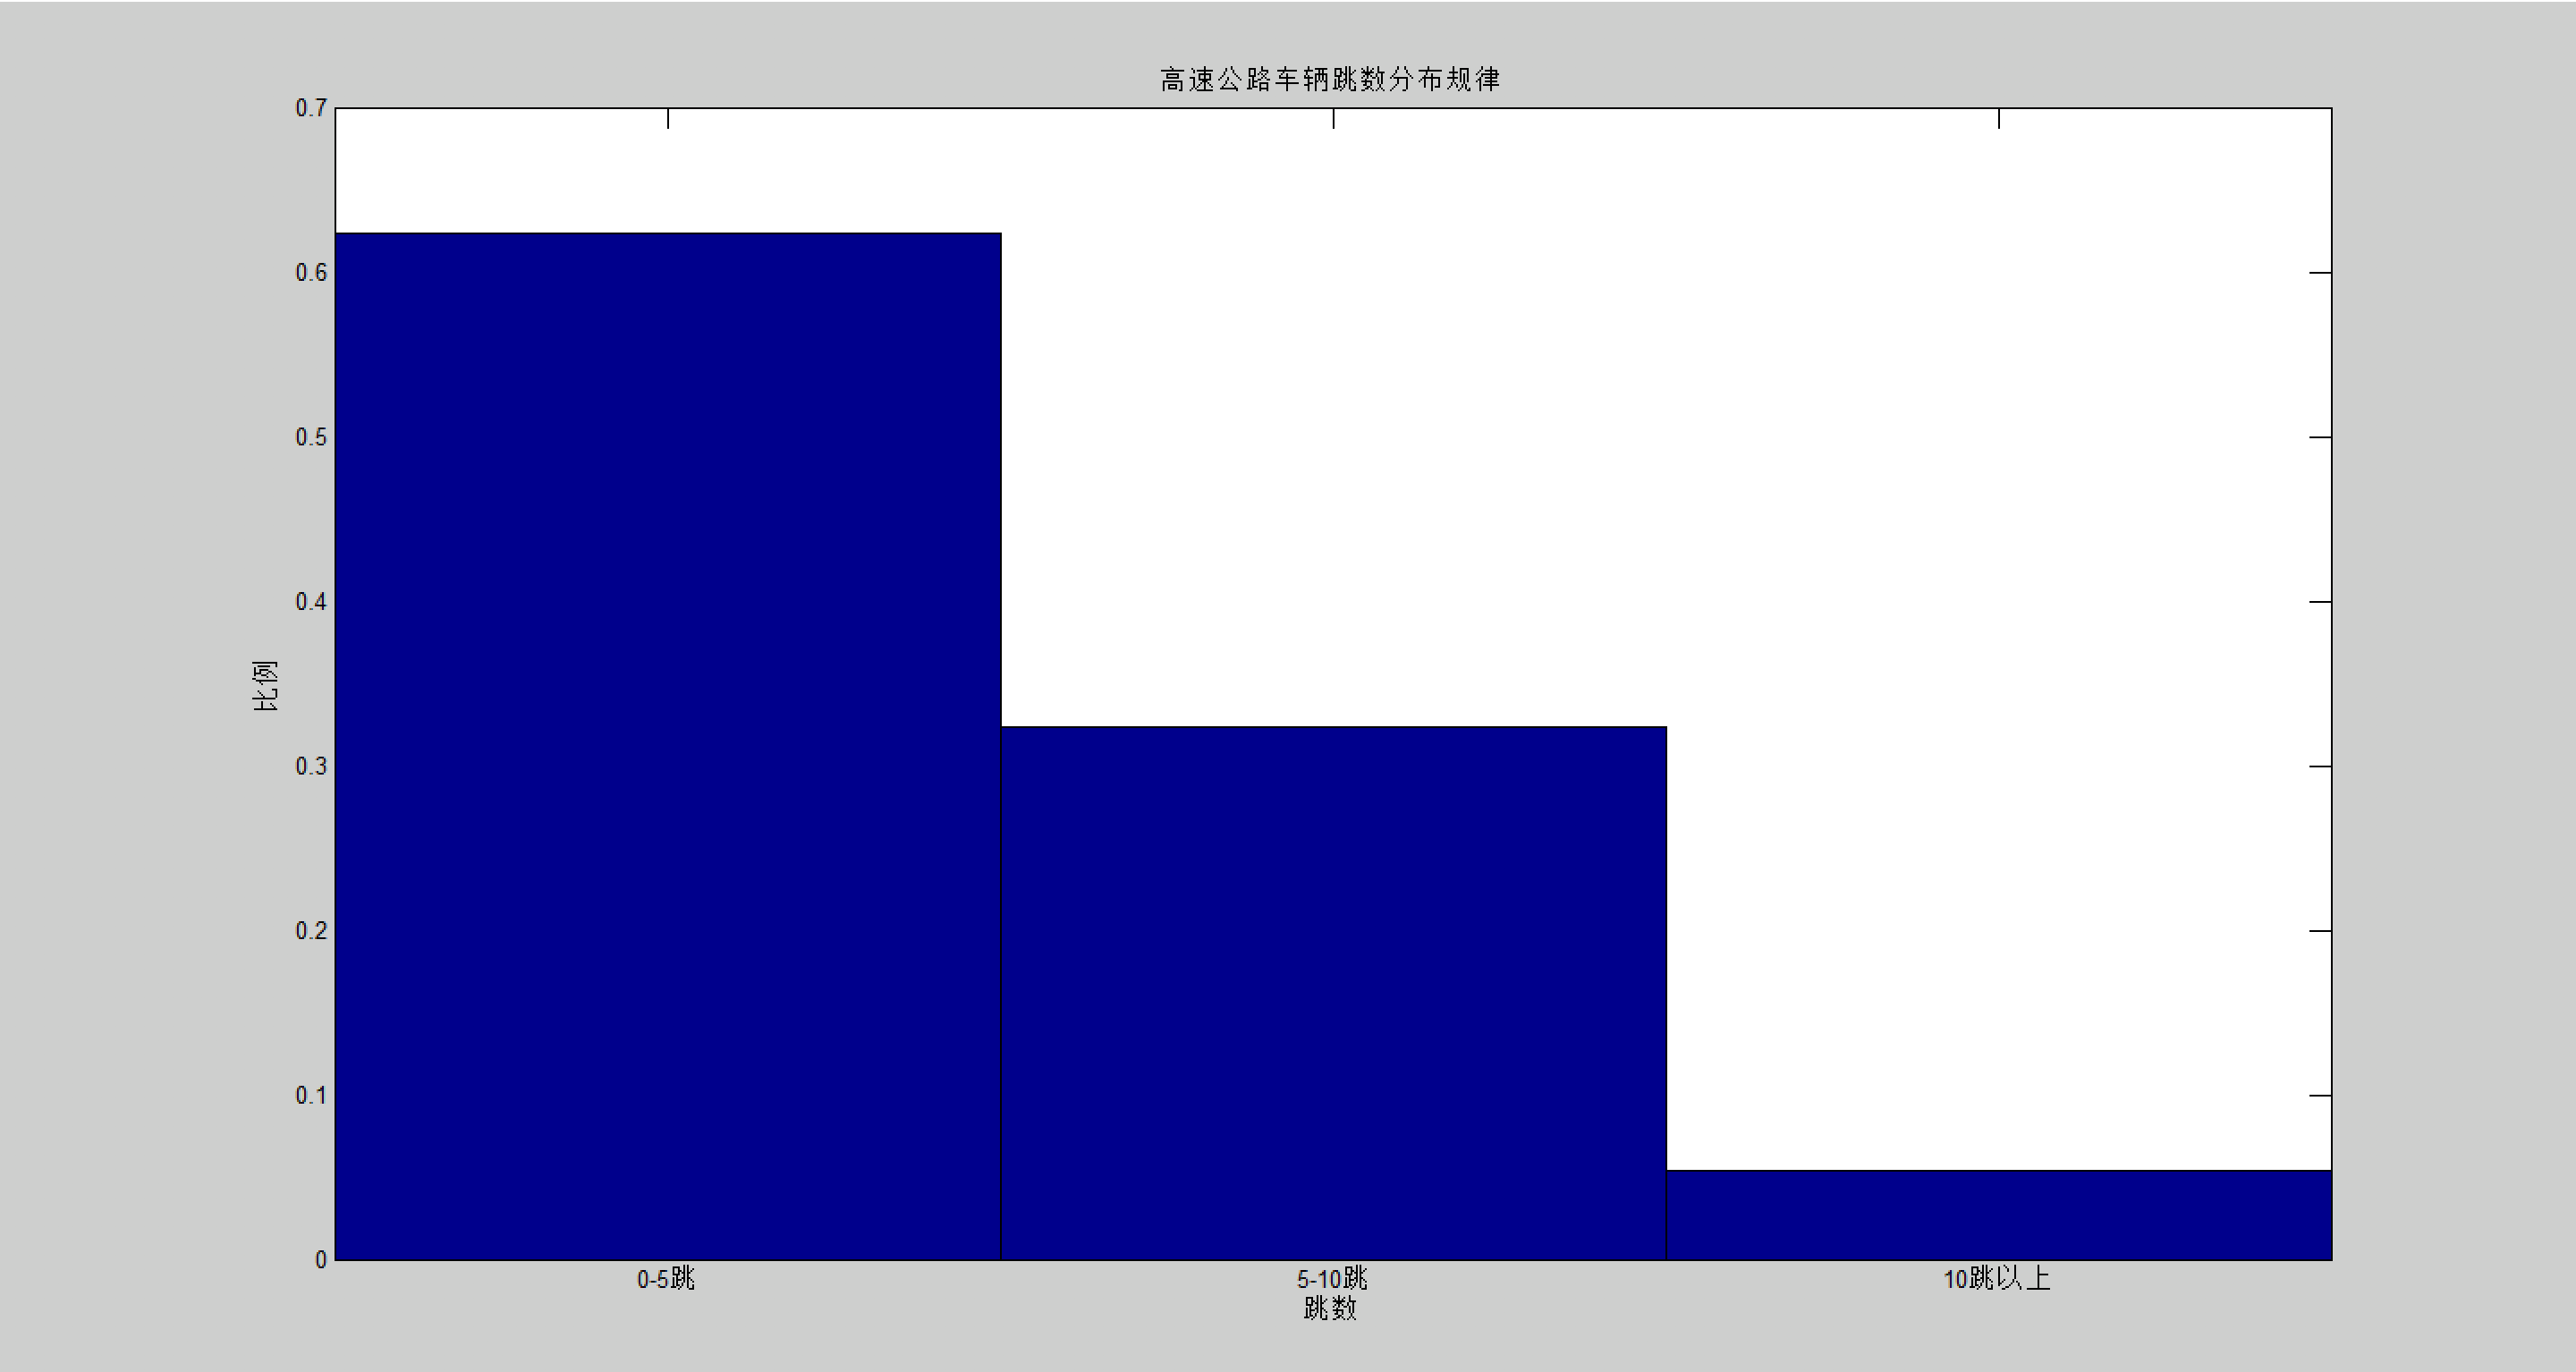
\includegraphics[width=4.4in]{picture/tiaoshu}
							\caption{高速公路车辆跳数分布图}
							\label{fig4}
						\end{minipage}%\
				\end{figure}

				为此,抽取某一天的高速公路O-D数据,将有O-D交流的收费站之间连线,流量越多,线的颜色越深,流量越少,线的颜色越浅。如图\ref{fig5},可以较直观的看出高速公路的社群特性。

				\begin{figure}[h]
				\centering
						\begin{minipage}{0.8\linewidth}
							\centering
							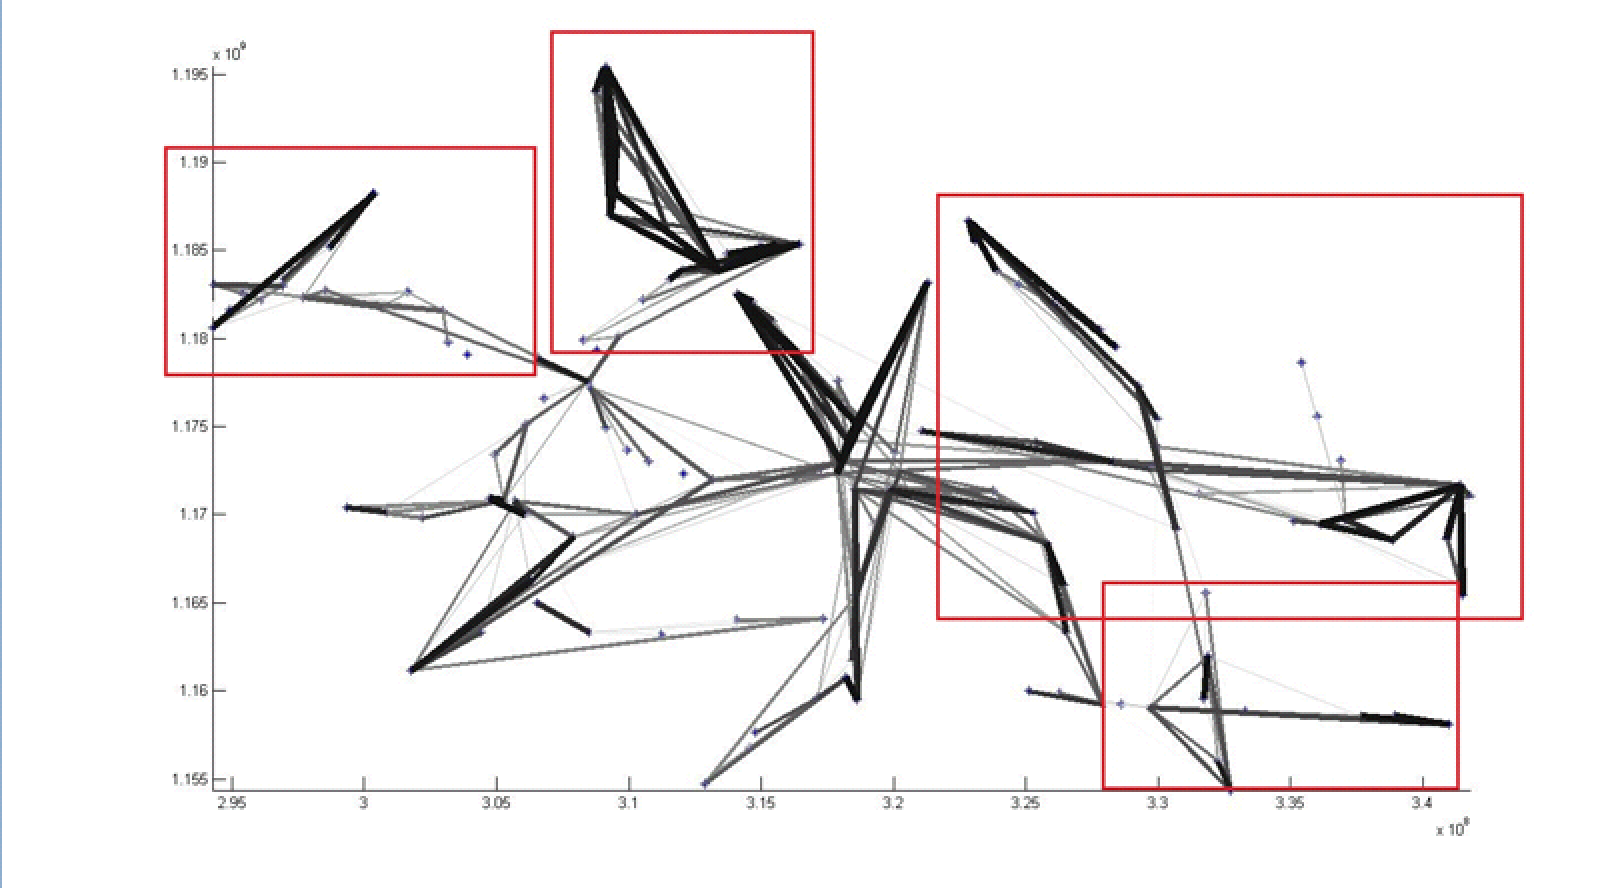
\includegraphics[width=4.4in]{picture/shequntexing}
							\caption{高速公路社群特性}
							\label{fig5}
						\end{minipage}%\
				\end{figure}
			%查重

				高速公路社群划分的目的是将整个高速公路拓扑结构分成一个个社群,使得社群内部交流尽量多,社群之间的交流尽量少,最终在各自社群分别计算关键路段,分治计算,最后进行合并,达到优化算法效率的目的。在此引入基于模块性优化的社群划分方法。

				复杂网络具有社群特性,高速公路属于复杂网络的一种。给定高速公路有向图$G=\{V,E\}$,其中V代表收费站(节点)的集合;E表示边的集合。定义社群$c=\{v_1,v_2,...v_m\}$,其中$v_i$是网络中的节点,即收费站或者交叉路口;社群集合$C=\{c_1,c_2,...c_u\}$;其中$v_i \in V$,${c_i}\bigcap {{c_j}}  = \emptyset$,$\sum\limits_{i = 1}^u {\sum\limits_{v \in {c_i}} v  = V}$。

				基于高速公路社群划分的关键路段挖掘算法主要采用分治思想,将一个难以直接解决的复杂问题,分割成一些规模较小的问题,逐个计算,分而治之。本文主要将路网分成一个个子路网,在子路网中分别计算关键路段,之后再用一定的方法进行合并。在此需要解决两个问题:

					1)如何分群:定制分群策略,使得不同社群之间的相互影响尽量小。

					2)如何合并:定制合并策略,将各个社群内部的计算结果合并到整个路网。

				传统的复杂网络社群划分方法中,大都是针对虚拟网络(如社交网络)进行研究。高速公路网络和虚拟网络有很大的不同。在虚拟网络中,两个点之间只要有交流,那就代表有边相连;在高速公路中,我们认为只要两个收费站有流量交流,即O-D不为0,那么这两个收费站之间就有边连接(不同于传统的路网定义)。但是这个边和其他的复杂网络如社交网络不同,社交网络中两个节点之间的空间距离定义为1跳,但是对于物理网络来说,两个节点之间的边具有实体距离。高速公路中路段之间的影响也会根据物理距离的变化而变化,这些都是传统方法中没有考虑到的。

				2004年,Newman和Girvan\parencite{NewmanBasic}提出了一个用于刻画网络社群结构优劣的量化标准,被称作模块化函数。简单的带权模块化函数定义如下:

				\begin{equation}
				Q = \frac{1}{{2m}}\sum\limits_{ij} {[{A_{ij}} - \frac{{{k_i}{k_j}}}{{2m}}]\delta ({c_i},{c_j})}
				\label{eq4}
				\end{equation}

				式\ref{eq4}中,$A_{ij}$表示节点$i$和节点$j$之间的边权;$k_i=\sum\limits_{j} {A_{ij}}$表示所有与节点i相连的边的边权和;$c_i$是指i所属的社群编号;如果$c_i=c_j$,那么$\delta (u,v)=1$,否则等于0;$m=\frac{1}{{2}}\sum\limits_{ij} {A_{ij}}$。

				模块化函数主要用于度量社群划分结构的优劣,现有的基于模块化函数的分群算法不适用于高速公路这种物理网络,并且在高速公路网络上出现了低分辨率特性和极端退化特性\parencite{Ren2014The}。
		\subsection{模型定义}

				针对现有研究的不足,结合高速公路的路网特性,提出一种新的面向高速公路的社群划分模型。首先定义模块化函数Q:

				\begin{equation}
				\vartriangle Q = [\frac{{\sum_{in} C  + 2{k_{i,in}}}}{{2m}} - {(\frac{{\sum_{tot} C  + {k_i}}}{{2m}})^2}] - [\frac{{\sum_{in} C }}{{2m}} - {(\frac{{\sum_{tot} C }}{{2m}})^2} - {(\frac{{{k_i}}}{{2m}})^2}] - L(i)
				\label{eq5}
				\end{equation}
				公式\ref{eq5}用于判断:当节点$i$从一个社群转移到另一个社群的时候,整体路网社群模块性的变化。节点的社群归属由$Q$变化的大小决定。式中,$\sum_{in} C$表示社群$C$内部的所有边的权重和;$\sum_{tot} C$表示所有与社群$C$中的节点相连的边的权重和;$k_{i,in}$表示$i$到$C$中所有节点之间的连线的权重和;$k_i$表示所有和节点i直接相连的边的权重和;m是路网中所有边的权重之和;$L(i)$是模型罚项,代表i转移社群后,不同社群之间交通流的变化。定义$L(i)$:

				\begin{equation}
				L(i)=\frac{{{k_{i,{c_1}}} - {k_{i,{c_2}}}}}{{{k_{{c_1},{c_2}}}}}
				\label{eq6}
				\end{equation}
				式\ref{eq6}中,${k_{i,{c_1}}}$表示路段i流向社群$c_1$的流量,$k_{i,{c_2}}$代表路段i流向社群$c_2$的流量,${{{k_{{c_1},{c_2}}}}}$表示社群$c_1$,$c_2$中所有节点之间的流量和。

				本文提出的模型中,边的权重不止与两个节点之间的流量有关,还与两个节点之间的物理距离有关。和传统复杂网络不同,节点之间的距离不再由节点之间的最短跳数决定,而是由节点之间的最短物理距离$L$决定:
				\begin{equation}
				L_{ij}=\sum\limits_{e \in E_{ij}} {e}
				\label{eq10}
				\end{equation}
				式\ref{eq10}中,$E_{ij}$是节点i和节点j之间的最短路径中路段的集合。定义边权重:


				\begin{equation}
				W_{ij}=\frac{f_{ij}}{L_{ij}*T}
				\label{eq11}
				\end{equation}

				为了解决传统社群划分中的低分辨率问题,本文中的社群划分方法也采用自底向上的聚类思想,首先定义每一个节点都是一个社群,社群集合$C=\{c_1,c_2,\dots,c_u\}$,路段集合$E=\{e_1,e_2,\dots,e_n\}$。初始情况下,$u=n$。在每次迭代过程中,遍历路段$E$,利用模块化函数$\vartriangle Q$,判断节点$e_i$所属的社群:
					$$\mathop{Max}\limits_{c_j\in C} (\vartriangle Q)$$
				式中,$\vartriangle Q$表示当路段$e_i$由原来的社群划分到社群$c_j$时,模块化函数的改变量。路段$|E|$经过一遍遍历后,形成一个新的社群集合$C^1=\{c_1^1,c_2^1,\dots,c_u^1\}$,结合社群集合和路段集合,进行下一轮遍历,直到收敛。

				传统方法中,社群划分具有极端退化特性,即最终结果无法收敛到某一个确定的最优解,而是会收敛到一个解集合中,在一定规模的解集中循环。比如说,假设社群划分已经收敛,在第$i$次迭代过程中,得到了社群集合$C^i$。$C^{i+1}\ne C^{i}$,但是在经过$k$次迭代后,$C^{i+k}=C^{i}$。实验表明,在高速公路上进行这样的社群划分,最终结果具有空间交叉特性,即不同的社群之间存在物理空间上的交叉(如图\ref{gulidian}),这种情况下不同社群之间的相互影响比较大。为了解决社群划分的空间交叉与极端退化问题,我们采用多变权值的思想,初始权值为$W_{ij}=\frac{f_{ij}}{L_{ij}*2}$,目标模型收敛后,记录本次迭代解集的规模k,变化权值$W_{ij}=\frac{f_{ij}}{L_{ij}*(2-0.1*l)}$(l为迭代次数),通过加大路段距离的权重,不断减少解集规模,改善社群之间空间交叉情况;为了加速收敛,结合模拟退火思想,定义退火温度为T,当轮迭代的解集数量为$k_i$,上轮迭代的解集数量为$k_{i-1}$。当$k_i<k_{i-1}$时,以概率$\frac {(k_{i-1}-k_i)}{T(k_{i-1})}$结束迭代。分群算法伪代码见Algorithm\ \ref{shequn}。

				\begin{algorithm}[h]
		        \caption{高速公路社群划分方法}  
		        \label{shequn}
		        \begin{algorithmic}[1] %每行显示行号  
		            \Require 高速车辆O-D数据,高速公路网络拓扑结构,最大社群节点数量
		            \Ensure 高速公路社群划分结果
		            \Function{Community}{$ODMatrix,G={V, E},B$}  
		                \State $res\gets [[\{0,0\},\{1,1\},\cdots,\{n,n\}]]$ 
		                \State $tmp\gets [\{\}]$
		                \State $pre\gets [[\{0,0\},\{1,1\},\cdots,\{n,n\}]]$ 
		                \State $k\gets 0$  
		                \State $l\gets 0$
		                \State $T\gets 100$  
		                \While{$|len(res)-len(pre)| \leqslant T$}
		                	\State $res=res[-1]$
		                	\State $pre=res$
		                	\While{$res[-1] \not\subset res[0:-1]$}
			                	\State $tmp\gets res[-1]$  
			                	\For{$i \in E $}  
			                		\For($C \in tmp \& |C| \le B$)
			                			\If{$\vartriangle Q > k$}  
				                        	\State $l\gets C$  
				                        	\State $k\gets {\vartriangle Q}$  
			                    		\EndIf	
			                		\EndFor
			                    	\State $tmp[l] \gets i$ 
			                	\EndFor
			                	\State $res \ add \ tmp$
		                	\EndWhile
		                	\State T--
		                \EndWhile  
		                \State \Return{$res$}  
		            \EndFunction  
		        \end{algorithmic}  
		    	\end{algorithm} 

		\subsection{基于社群划分的关键路段求解}
				基于已经分群的高速公路网络,提出关键路段挖掘方法。

				本节算法的核心思想是分治法。首先分割社群,将每个社群看作独立的路网。在每个社群内部,用贪心算法选出关键路段,记录每个关键路段被处理后,路段通行效率的增量$\vartriangle L$。忽略不同社团的关键路段之间的相互影响。这样,分治法的合并问题被归类于投资问题。

				投资问题的定义如下:定义资产总额为$B$,总共有$\{X_1,X_2,\dots,X_u\}$ \ u种货物,每种货物可以投资$[0-B]$份资源。$g(y*X_{i})$表示当货物$X_i$投资量为$y$时,它所带来的收益。本节中,定义关键路段的数目为B,社团$i$由$X_i$表示,每个社团中,用$g(t*X_{i})$计算改造关键路段造成的影响。在此提出目标模型:

				\begin{align}
				 &Q=Max(\sum\limits_{i = 1}^u {g({y}*{X_i})})   \label{fenzhi-merge} \\
				 &Subject \  to. \  \left\{ {\begin{array}{*{20}{c}}
					  {\sum\limits_{i = 1}^u {{y}}  \leqslant B} \\ 
					  {{x_i} \geqslant 0} 
				\end{array}} \right.
				\end{align}

				\ref{fenzhi-merge}属于投资问题,可以利用动态规划,在多项式时间内求解。求解步骤如下:

				定义$f_k (x)$为前k个社团投入x份资源时,高速公路通行效率的最大提升量,首先赋初始值:$f_0(x)=0$;$f_k(0)=0$;$f_1(x)=g(x*X_{1})$。递推公式:
					$$f_i (j)=\mathop {{\text{Max}}}\limits_{0 \leqslant y \leqslant j} (CMatrix[i][y]+f_{i-1} (j-y))$$

				公式中,CMatrix矩阵表示当社团i投资y条路段时,路网通行效率的增加量;y表示本社团中投资路段的数量,根据y和贪心算法结果,可以推算出具体路段。当$k=2$时,$CMatrix$矩阵已知,$f_1(x)$全部已知,据此可以推算出所有$f_2(x)$的值。递推,依次得到$f_3(x),\dots,f_u(x)$的值,结合$f_u(x)$中y的值,根据贪心算法,获取关键路段,反向递推,得到最终关键路段的集合。
				动态规划伪代码:

				\begin{algorithm}[h]
		        \caption{关键路段挖掘方法求解}  
		        \label{touzi}
		        \begin{algorithmic}[1] %每行显示行号  
		            \Require 每个社团中选取不同路段的收益,高速公路网络社团结构,最大社群节点数量
		            \Ensure 高速公路关键路段集合
		            \Function{Community}{$CMatrix,C={c_1,c_2,...,c_u},B$}  
		                \State 定义$f_k (x)$:当前k个社团投入x份资源时,最大的通行效率提升量
		                \State $f_0 (x)\gets 0$
		                \State $f_k (0)\gets 0$
		                \State $f_1 (x)\gets CMatrix[1][x]$
		                \State $i=j=1$
		                \While{$i \leqslant u$}
		                	\While{$j\leqslant B$}
		                		\State $f_i (j)=\mathop {{\text{Max}}}\limits_{0 \leqslant y \leqslant j} (CMatrix[i][y]+f_{i-1} (j-y))$
		                		\State $j=j+1$
		                	\EndWhile
		                	\State $i=i+1$
		                \EndWhile  
		                \State \Return{$res$}  
		            \EndFunction  
		        \end{algorithmic}  
		    	\end{algorithm} 

		    	其中,路段收益矩阵CMatrix:

				\[\begin{array}{*{20}{c}}
				  {{c_{11}}}&{{c_{12}}}& \cdots &{{c_{1B}}} \\ 
				  {{c_{21}}}&{{c_{22}}}& \cdots &{{c_{2B}}} \\ 
				   \vdots & \vdots & \ddots & \vdots  \\ 
				  {{c_{u1}}}&{{c_{u2}}}& \cdots &{{c_{uB}}} 
				\end{array}\]
				
				矩阵中,$c_{ij}$表示第i个社群中,选取j条关键路段进行资源投放后,高速公路网络通行效率的提升量。这一数据由贪心算法在每个社群分别求得。

	\section{实验及结果}
		本章节出了针对每一种方法的有效性做出实验,并将基于高速公路社群划分方法的实际效果与通过枚举得到的最优解进行对比。

		基本的社群划分存在分辨率限制和极端退化特性。分辨率限制是指社群划分方法无法发现小于一定规模的社群,极端退化特性是指最终的社群划分结果会收敛于指数数量级的高分解决方案,而不是指向一个或少量最优解。Newman\parencite{NewmanFast}采用一种方法解决低分辨率问题:初始化时,将每一个节点看作一个独立的社群,之后根据模块化函数不断循环修正节点的所属社群。这个方法用在高速公路上时,虽然解决了低分辨率社群无法发现的问题,但是最终会产生一系列孤立点(如图\ref{gulidian}),这不符合社群划分的初衷。而且最终结果也没有避开极端退化特性,最终的社群划分结果在一个非常大的解空间中循环。

			\begin{figure}[h]
			\centering
					\begin{minipage}{0.8\linewidth}
						\centering
						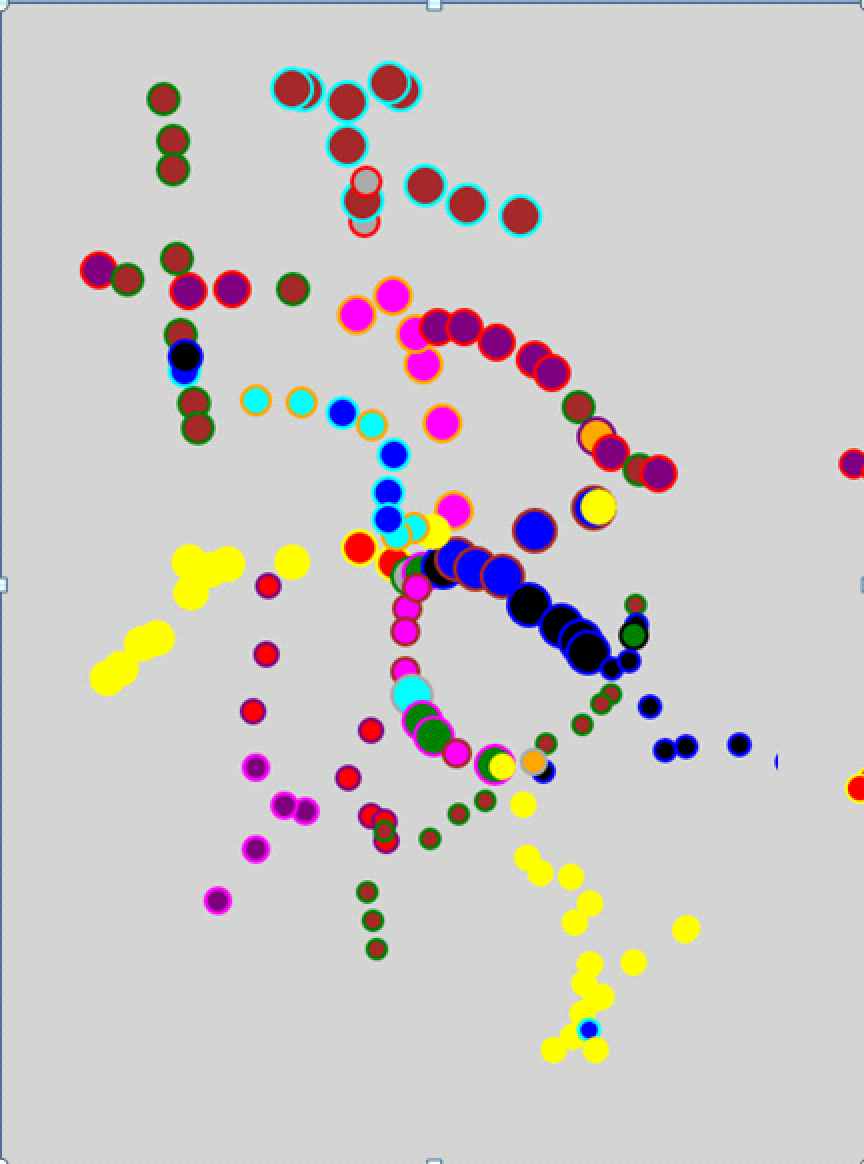
\includegraphics[width=3in]{picture/liuliangbianquan}
						\caption{基于模块化函数的社群划分方法}
						\label{gulidian}
					\end{minipage}
			\end{figure}

		图\ref{gulidian}给出了基本的基于模块化函数的分群结果,首先需要指出:使用基础方法的分群结果收敛于一个具有一千多个解的解集合。最终分群结果会在这些解集合内循环。由图我们可以看出两个问题:

		1)存在很多未被分群的孤立点。

		2)很多社群存在物理意义上的交叉收费站。

		孤立点的产生原因有两个,一是这个收费站本身流量较小,与其他站点交流不多;二是这个站点与其他站点之间的交流较为平均,站点不断流动于不同的社团中。图\ref{fenqun2}是基于公式\ref{eq5}的社群划分结果,该图由几百个社群划分解组成的解集中选出,由图可以看出加入物理路经长度的情况下,可以在一定程度上消除孤立点,并且将高速公路划分成较为清晰的几类。但是我们发现仍旧有少量社群,存在物理层面的相互交叉情况,而这种情况不符合高速公路这种物理网络的社群划分特点。

				\begin{figure}
				\begin{minipage}{0.5\linewidth}
					\centering
					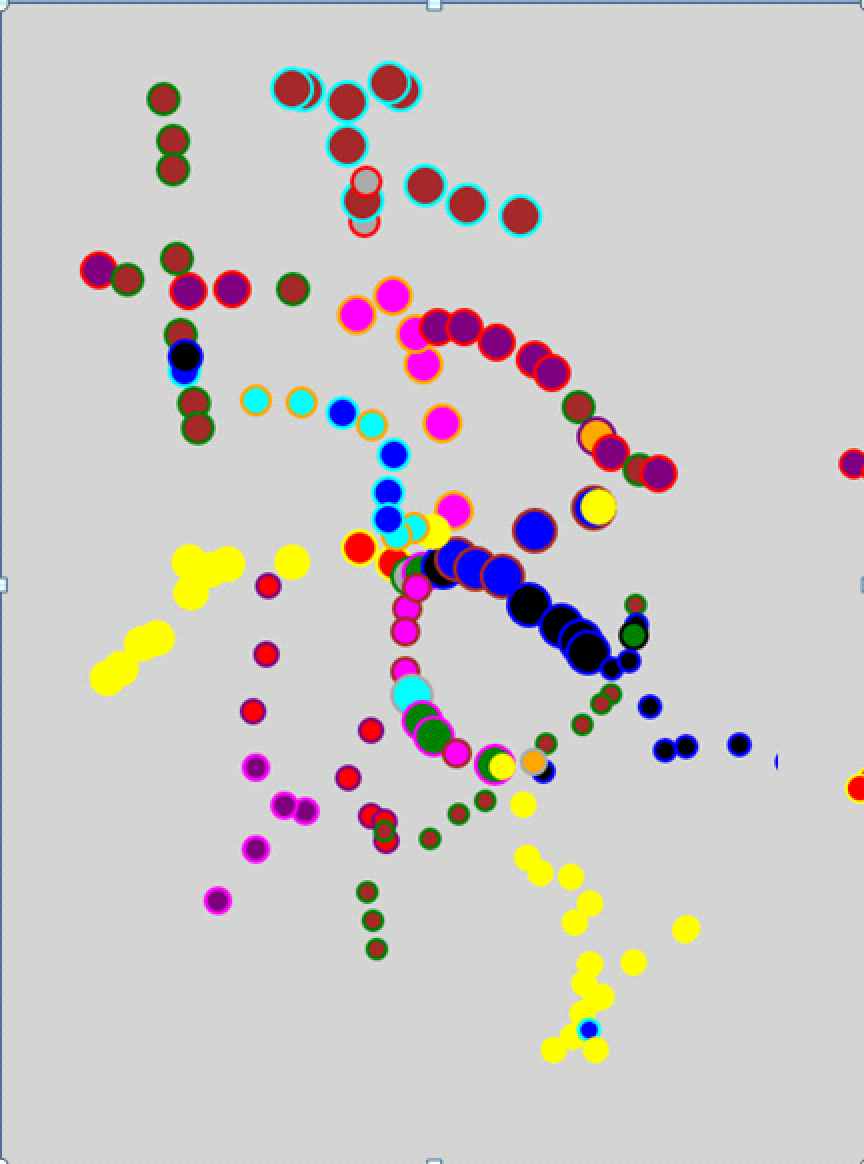
\includegraphics[width=2.2in]{picture/liuliangbianquan}
					\caption{基于模块化函数的社群划分方法}
					\label{fenqun1}
				\end{minipage}%
				\begin{minipage}{0.5\linewidth}
					\centering
					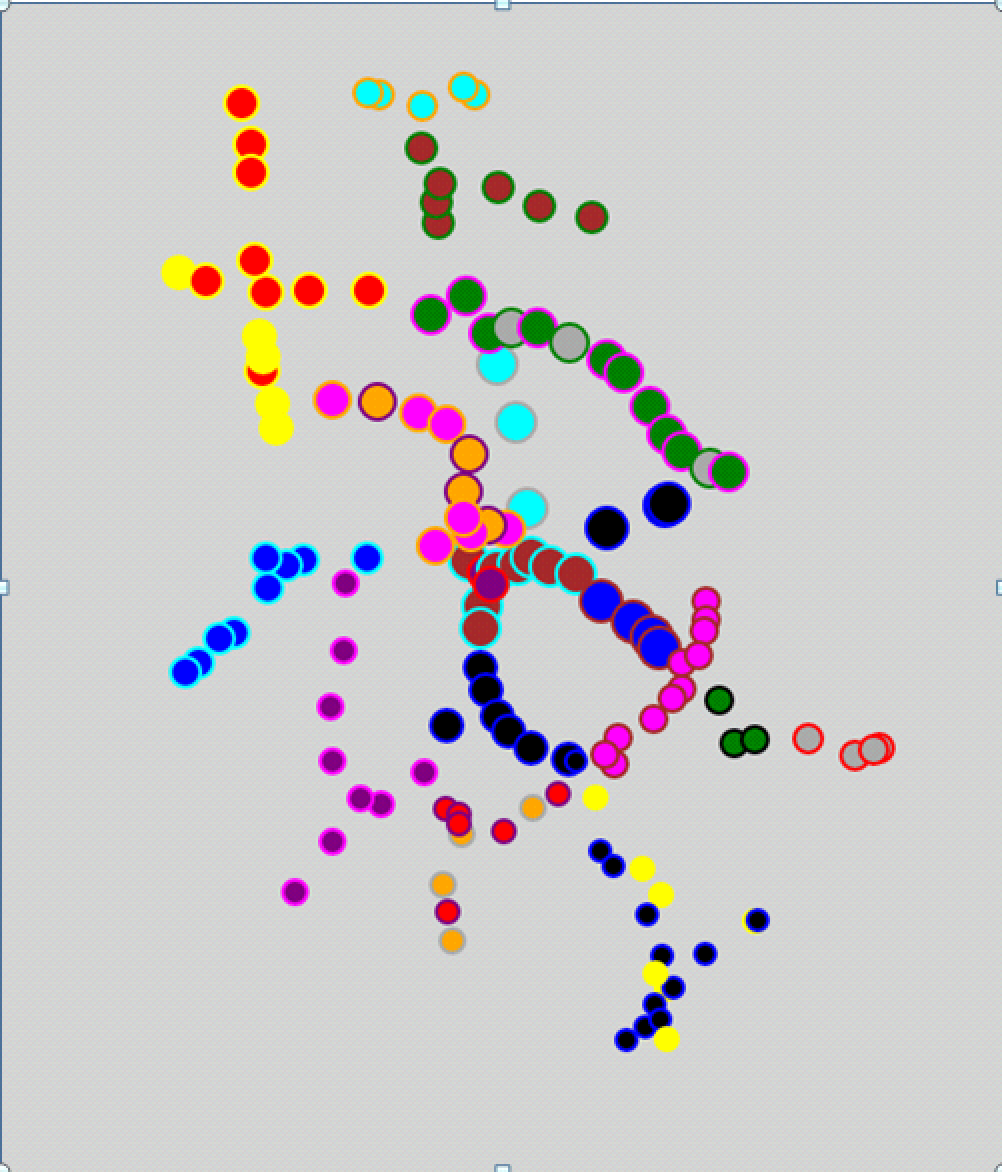
\includegraphics[width=2.5in]{picture/xiaochuguli}
					\caption{结合物理路网特性的社群挖掘}
					\label{fenqun2}
				\end{minipage}
				\end{figure}

		经过数据分析,出现图\ref{fenqun2}中不同社群内部的节点之间存在物理上的交叉情况的原因是——不同社群节点之间的流量差远大于节点之间的距离差。直接将具有交叉节点的社群进行合并虽然简单有效,但是不具有更大规模的适应性,这种方法得到的社群划分效果得不到保证,而且有可能出现过大的社团,不符合社群划分的目的。图\ref{fenqun3}给出了基于模拟退火方法的迭代分群方法结果,该结果最终收敛于由5个结果组成的结果集,基本消除所有孤立点与社群交叉节点。


				\begin{figure}
				\centering
				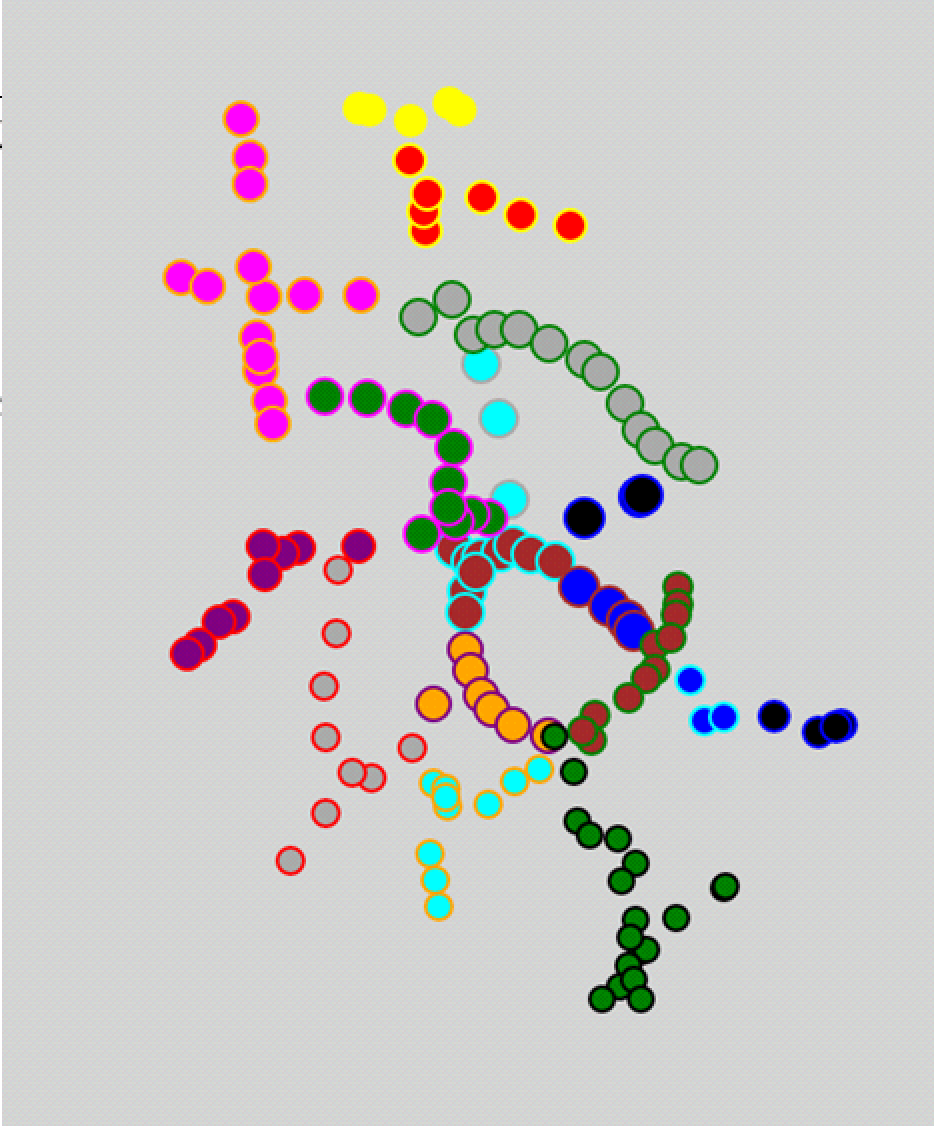
\includegraphics[width=3in]{picture/fenqunjieguo}
				\caption{结合路段距离的变权社群挖掘结果}
				\label{fenqun3}
				\end{figure}

		根据公式\ref{eq4}给出的模块化函数Q,表\ref{table10}给出了不同社群方法模块化的效果。可以看出将边权与物理距离结合考虑后,模块化效果得到了显著提高;虽然模拟退火方法的时间消耗较大,但是它提供了符合物理网络的分群结果,减少不同社群之间的交叉节点,将不同社群之间节点的相互影响降到最低。

				\begin{table}[h]
				\centering
				\begin{tabular}{|c|c|c|c|}
				\hline
				\hline
				   &   基于流量划分 &   基于流量/距离划分 &   基于变化距离的模拟退火  \\
				\hline
				  模块化效果 &   -1321.21 &   -1025.50 &   -1182.84  \\
				\hline
				  算法效率 &   1min &  30s   &   1.5min  \\
				\hline
				  收敛度 &   $10^3$ &   $10^2$ &   $0-10$  \\
				\hline
				\end{tabular}
				\caption{不同社群划分方法效果对比}
				\label{table10}
				\end{table} 



		图\ref{fenqunend}给出了一天时间内,基于分群算法和简单贪心方法的对比试验;图\ref{end}给出了在一周时间内两种方法的对比试验。和上一章节一样,横坐标表示时间,纵坐标表示路网通行效率的绝对值(路网通行时间)。由图可以看出,简单贪心算法和基于分群算法的关键路段挖掘算法之间的误差较为平稳,并且一直维持在一个较低的水平线上。由图可以看出,分群算法可以在和统计算法相似的时间复杂度上,得到比统计算法优秀的解集。

				\begin{figure}
				\begin{minipage}{0.5\linewidth}
					\centering
					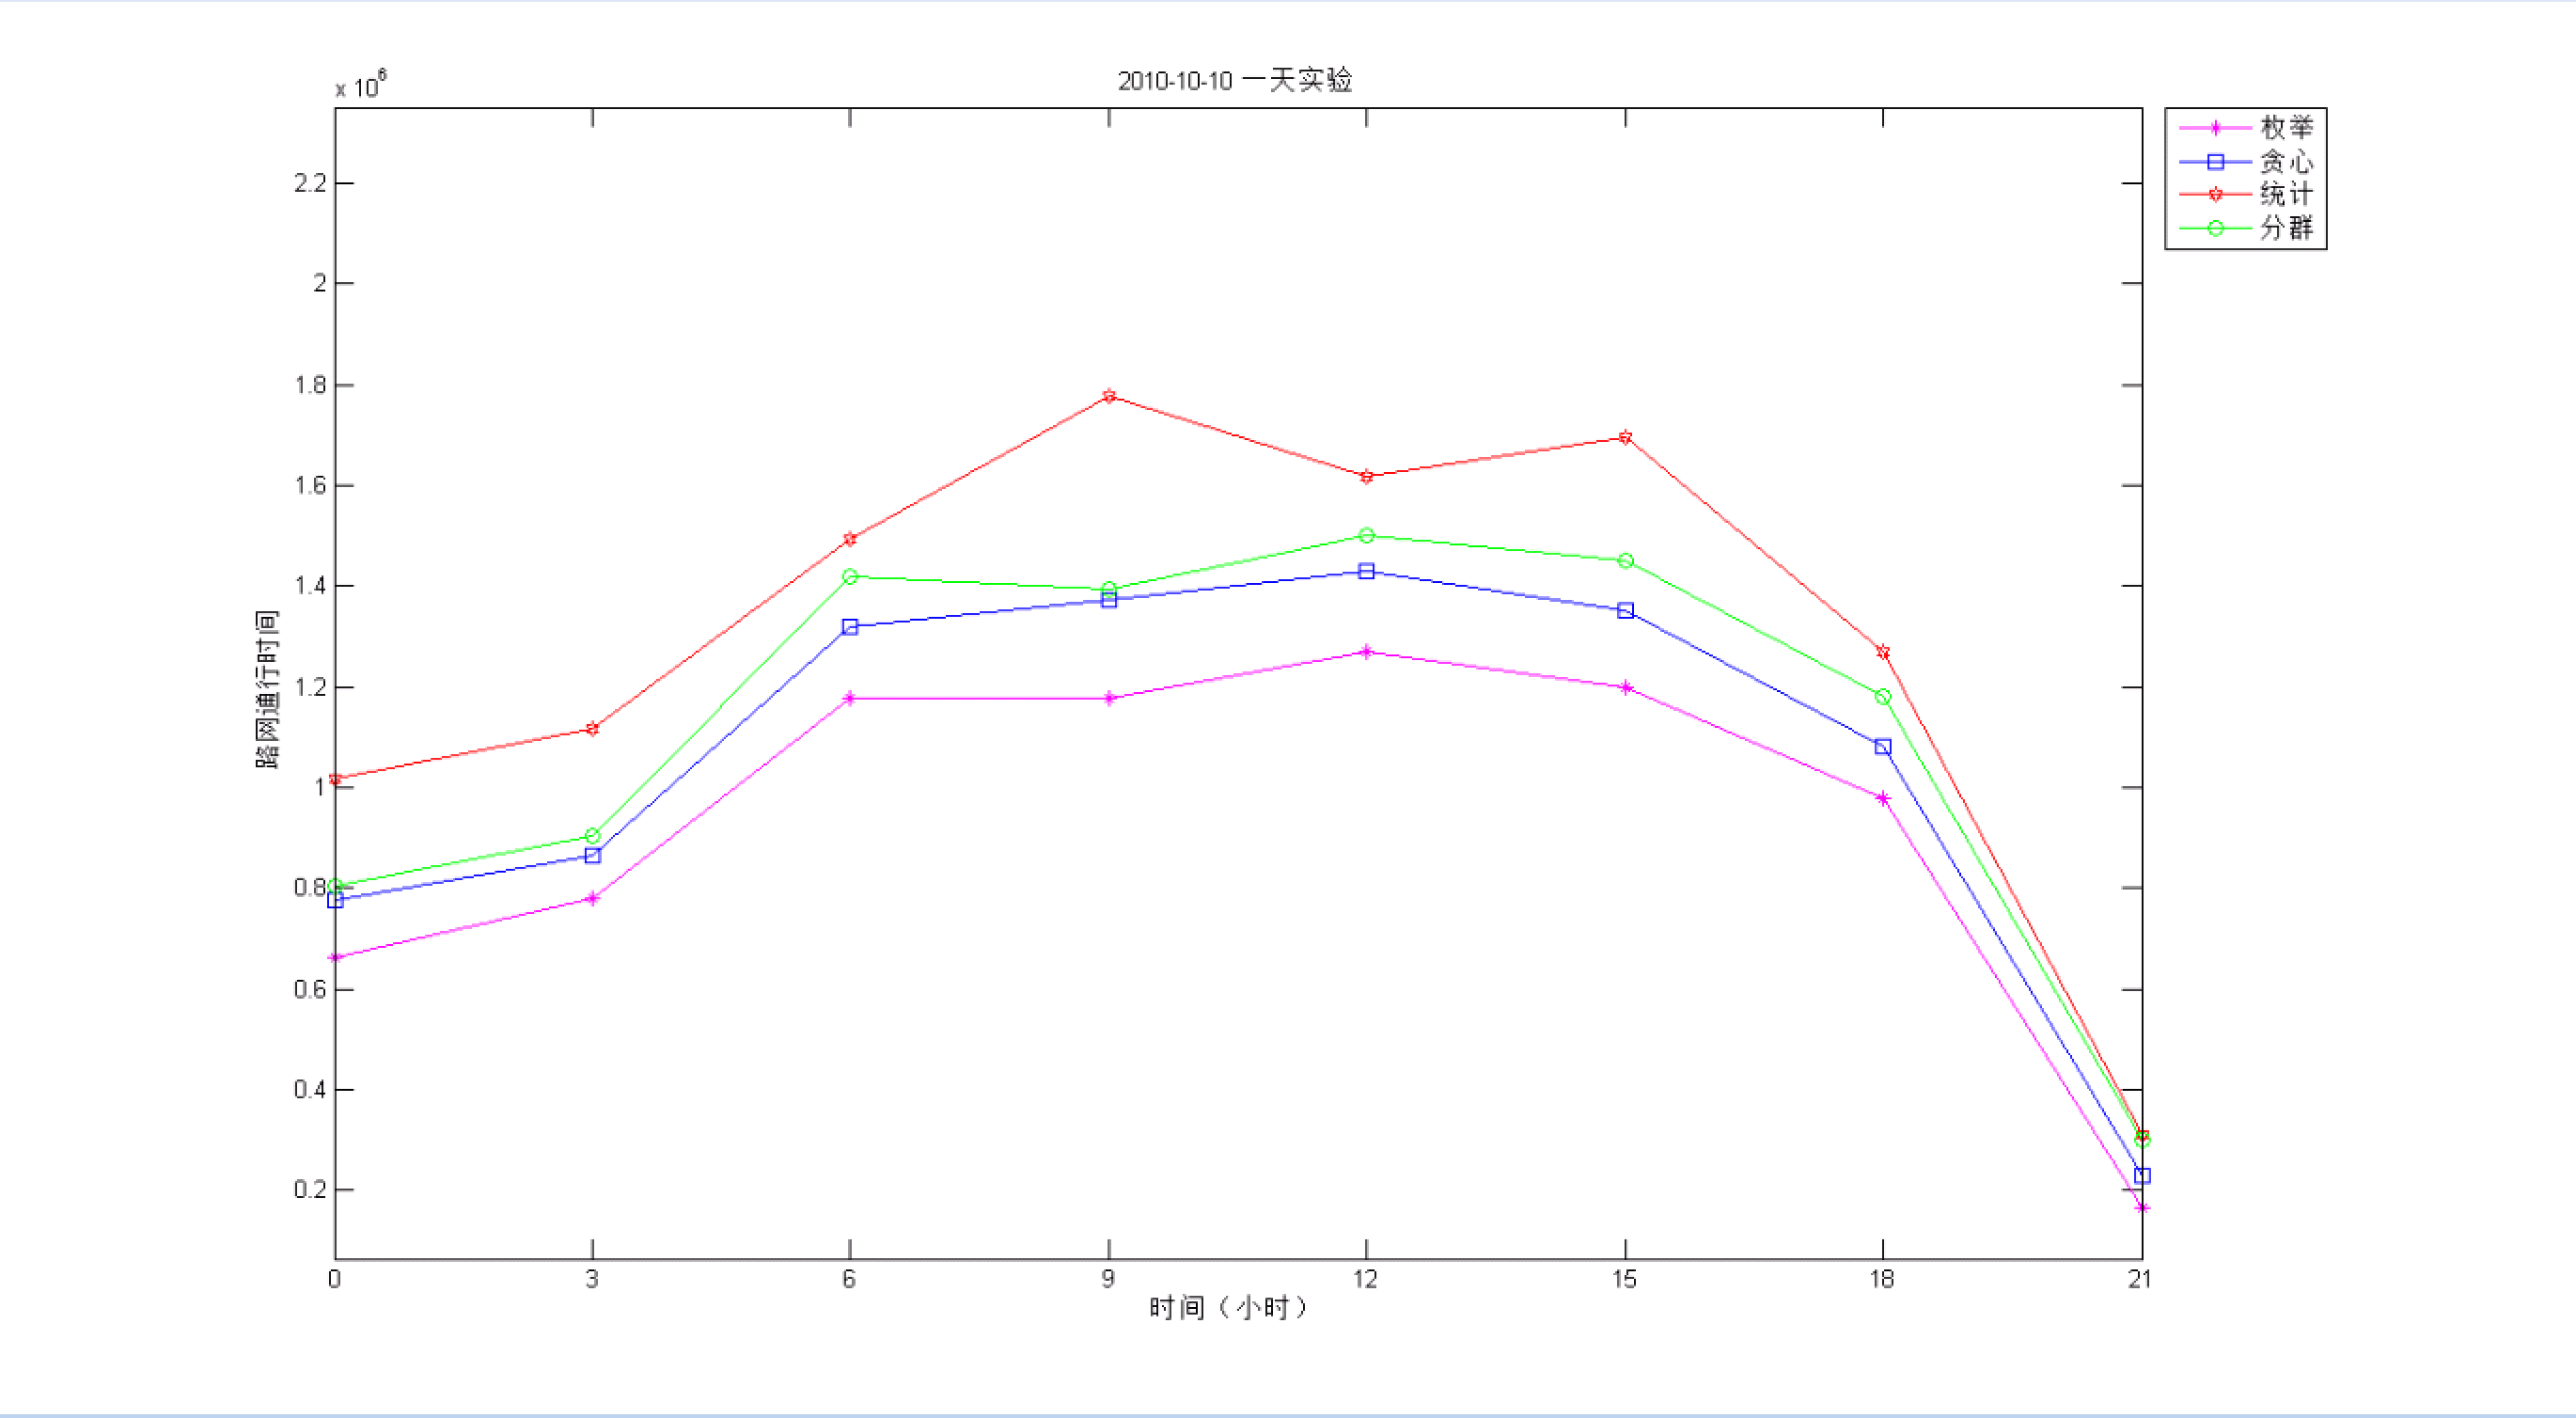
\includegraphics[width=3in]{picture/fenqunend}
					\caption{对比实验:以1h为区间}
					\label{fenqunend}
				\end{minipage}%
				\begin{minipage}{0.5\linewidth}
					\centering
					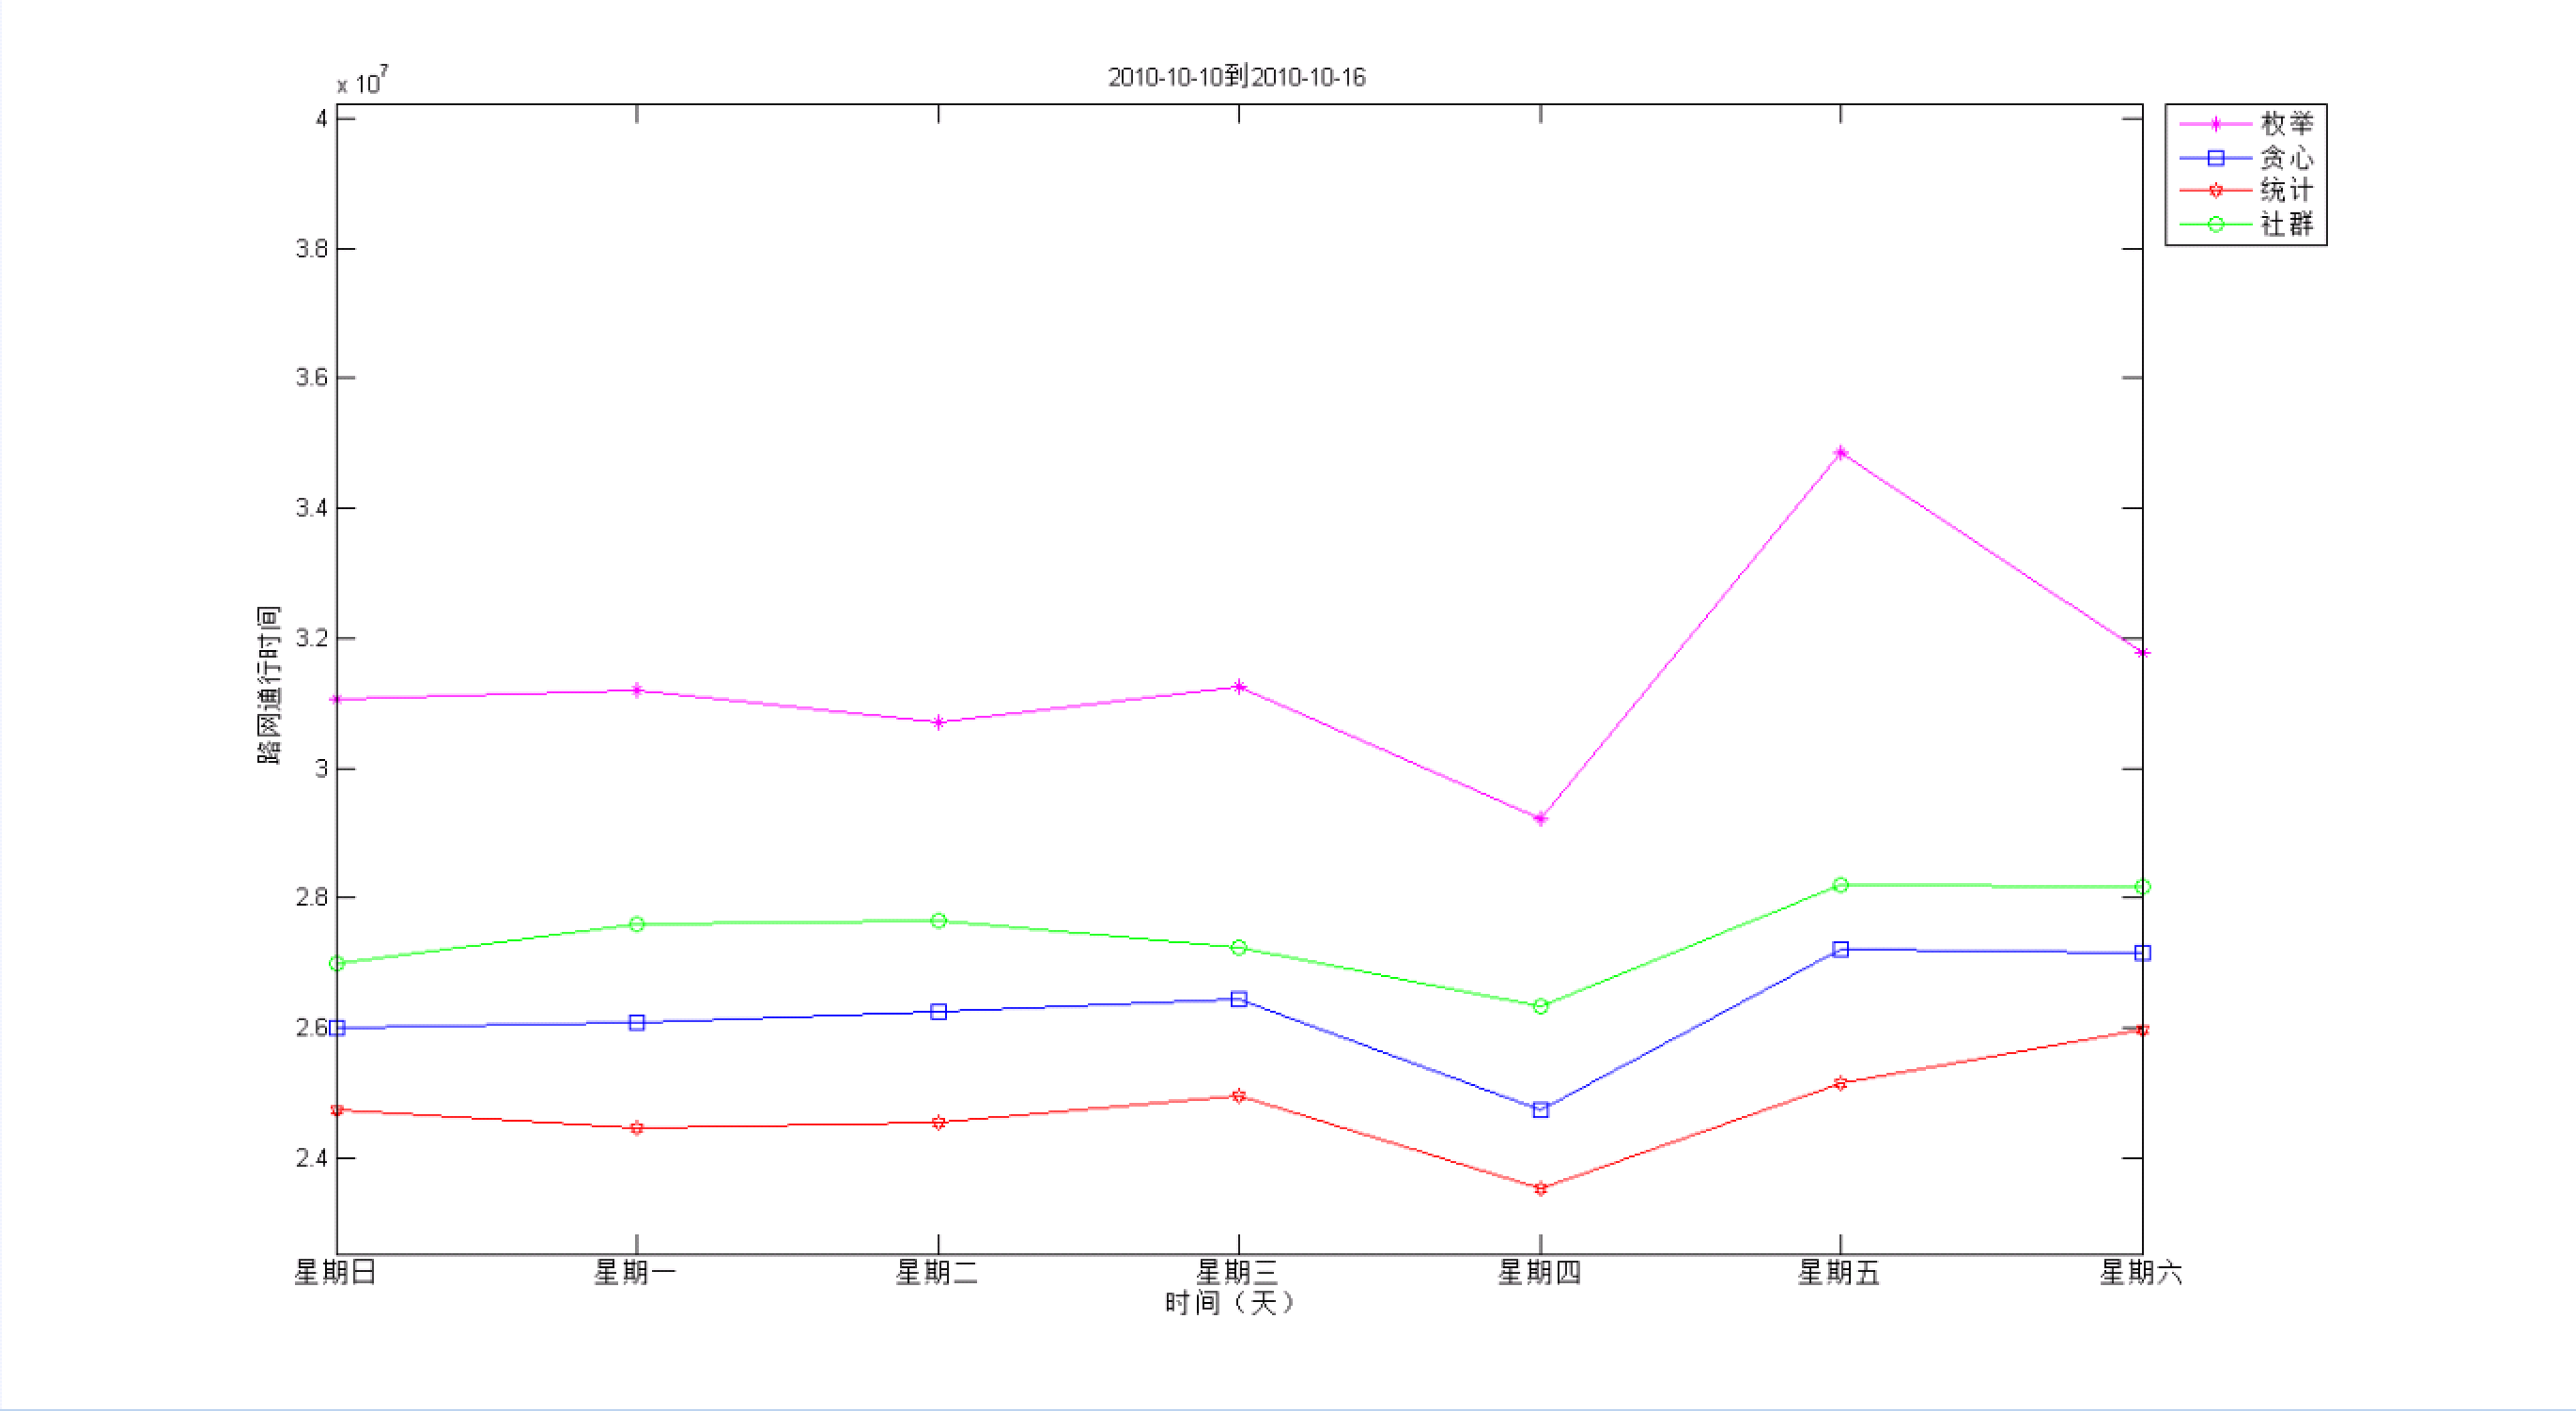
\includegraphics[width=3in]{picture/end}
					\caption{对比实验:以1d为区间}
					\label{end}
				\end{minipage}
				\end{figure}

		下图给出不同方法选出的关键路段集合,图\ref{jihe1}给出了枚举方法选出的关键路段集合,图\ref{jihe2}给出了简单贪心算法给出的关键路段集合,图\ref{jihe3}给出了结合社群划分的关键路段识别算法的结果,图\ref{jihe4}给出了基于统计学的关键路段集合。观察图\ref{jihe1}和图\ref{jihe2},发现两者选取的关键路段具有很强的相似性。

				\begin{figure}
				\begin{minipage}{0.5\linewidth}
					\centering
					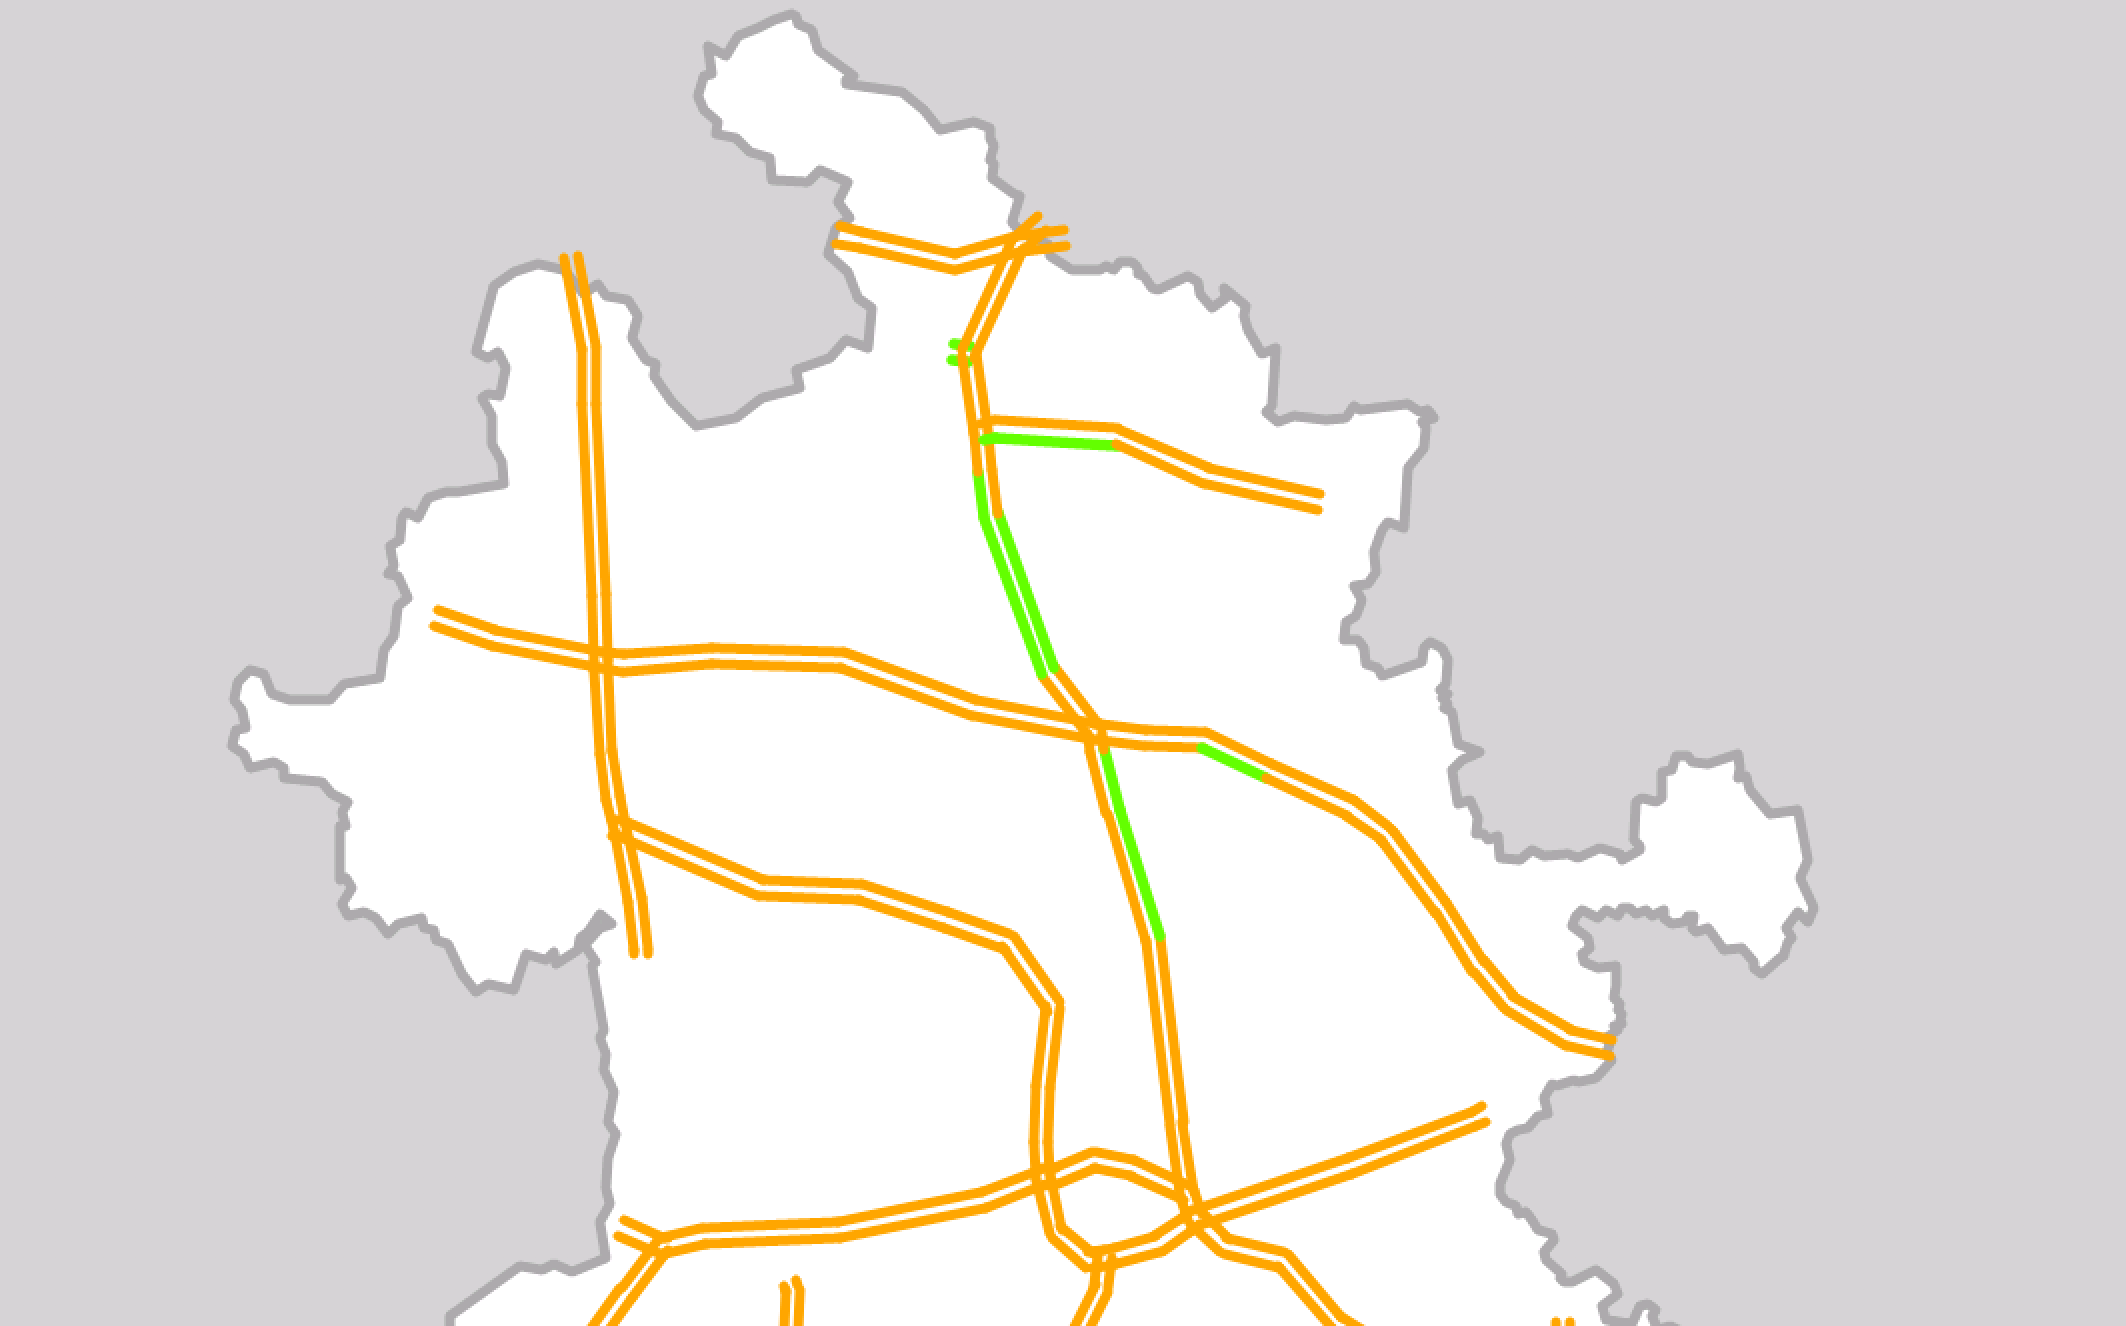
\includegraphics[width=3in]{picture/meiju}
					\caption{枚举求得关键路段}
					\label{jihe1}
				\end{minipage}%
				\begin{minipage}{0.5\linewidth}
					\centering
					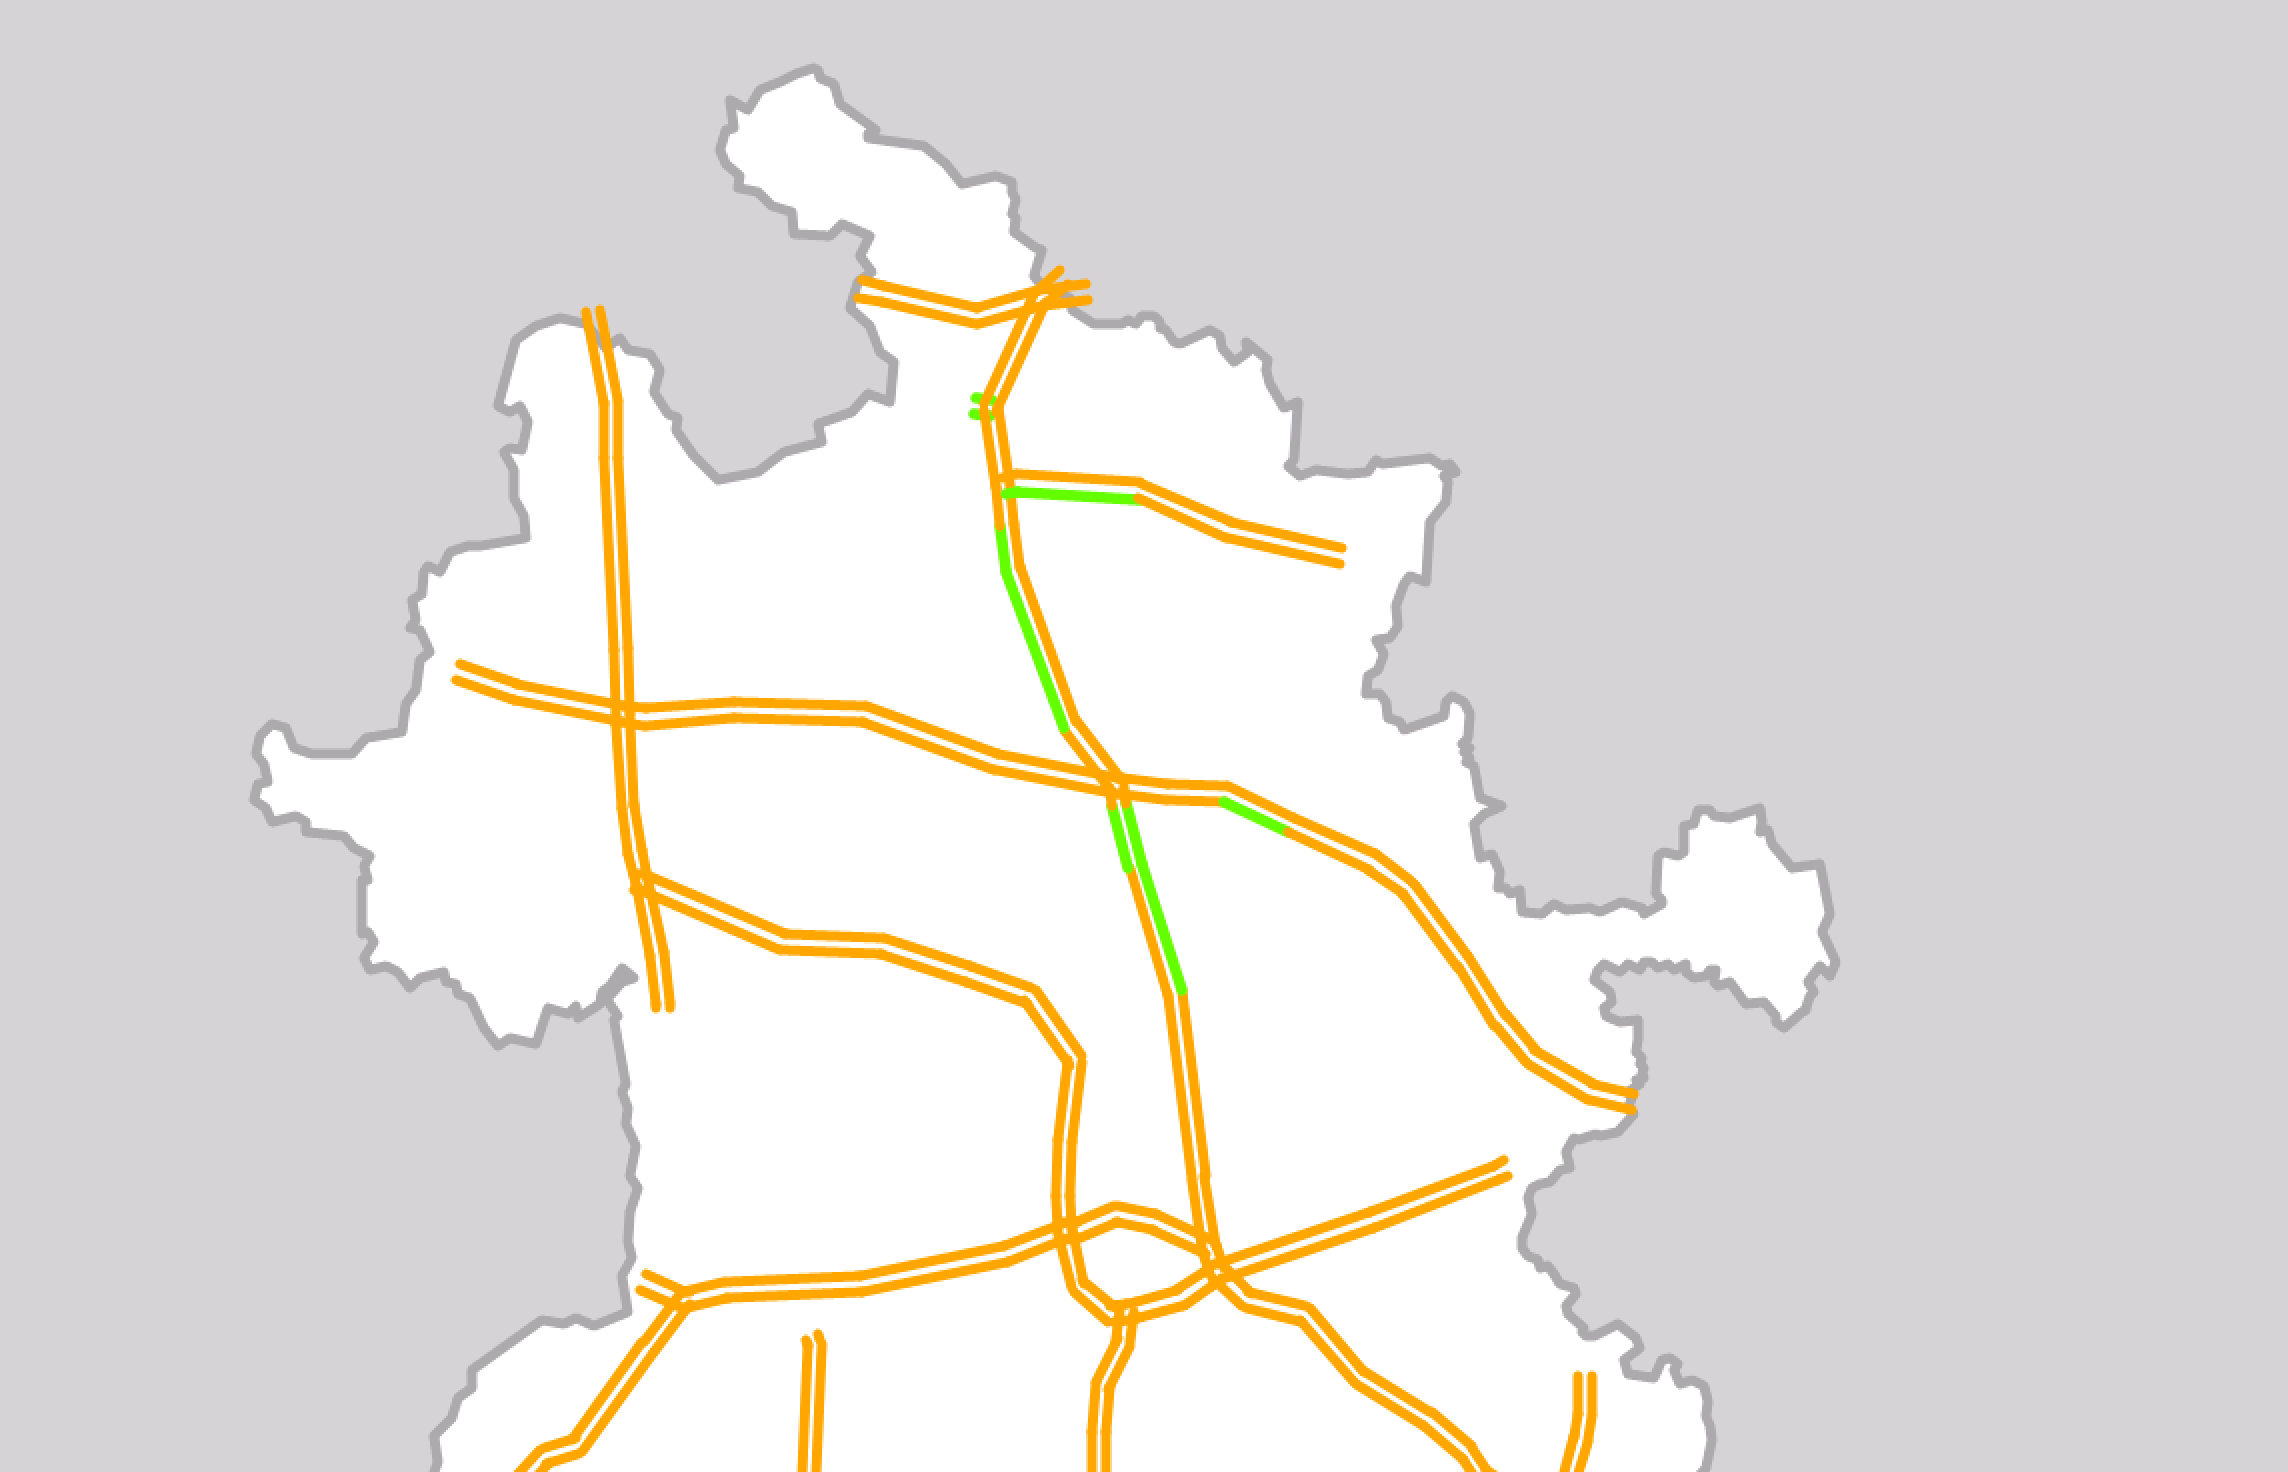
\includegraphics[width=3in]{picture/tanxin}
					\caption{贪心求得关键路段}
					\label{jihe2}
				\end{minipage}
				\end{figure}

				\begin{figure}
				\begin{minipage}{0.5\linewidth}
					\centering
					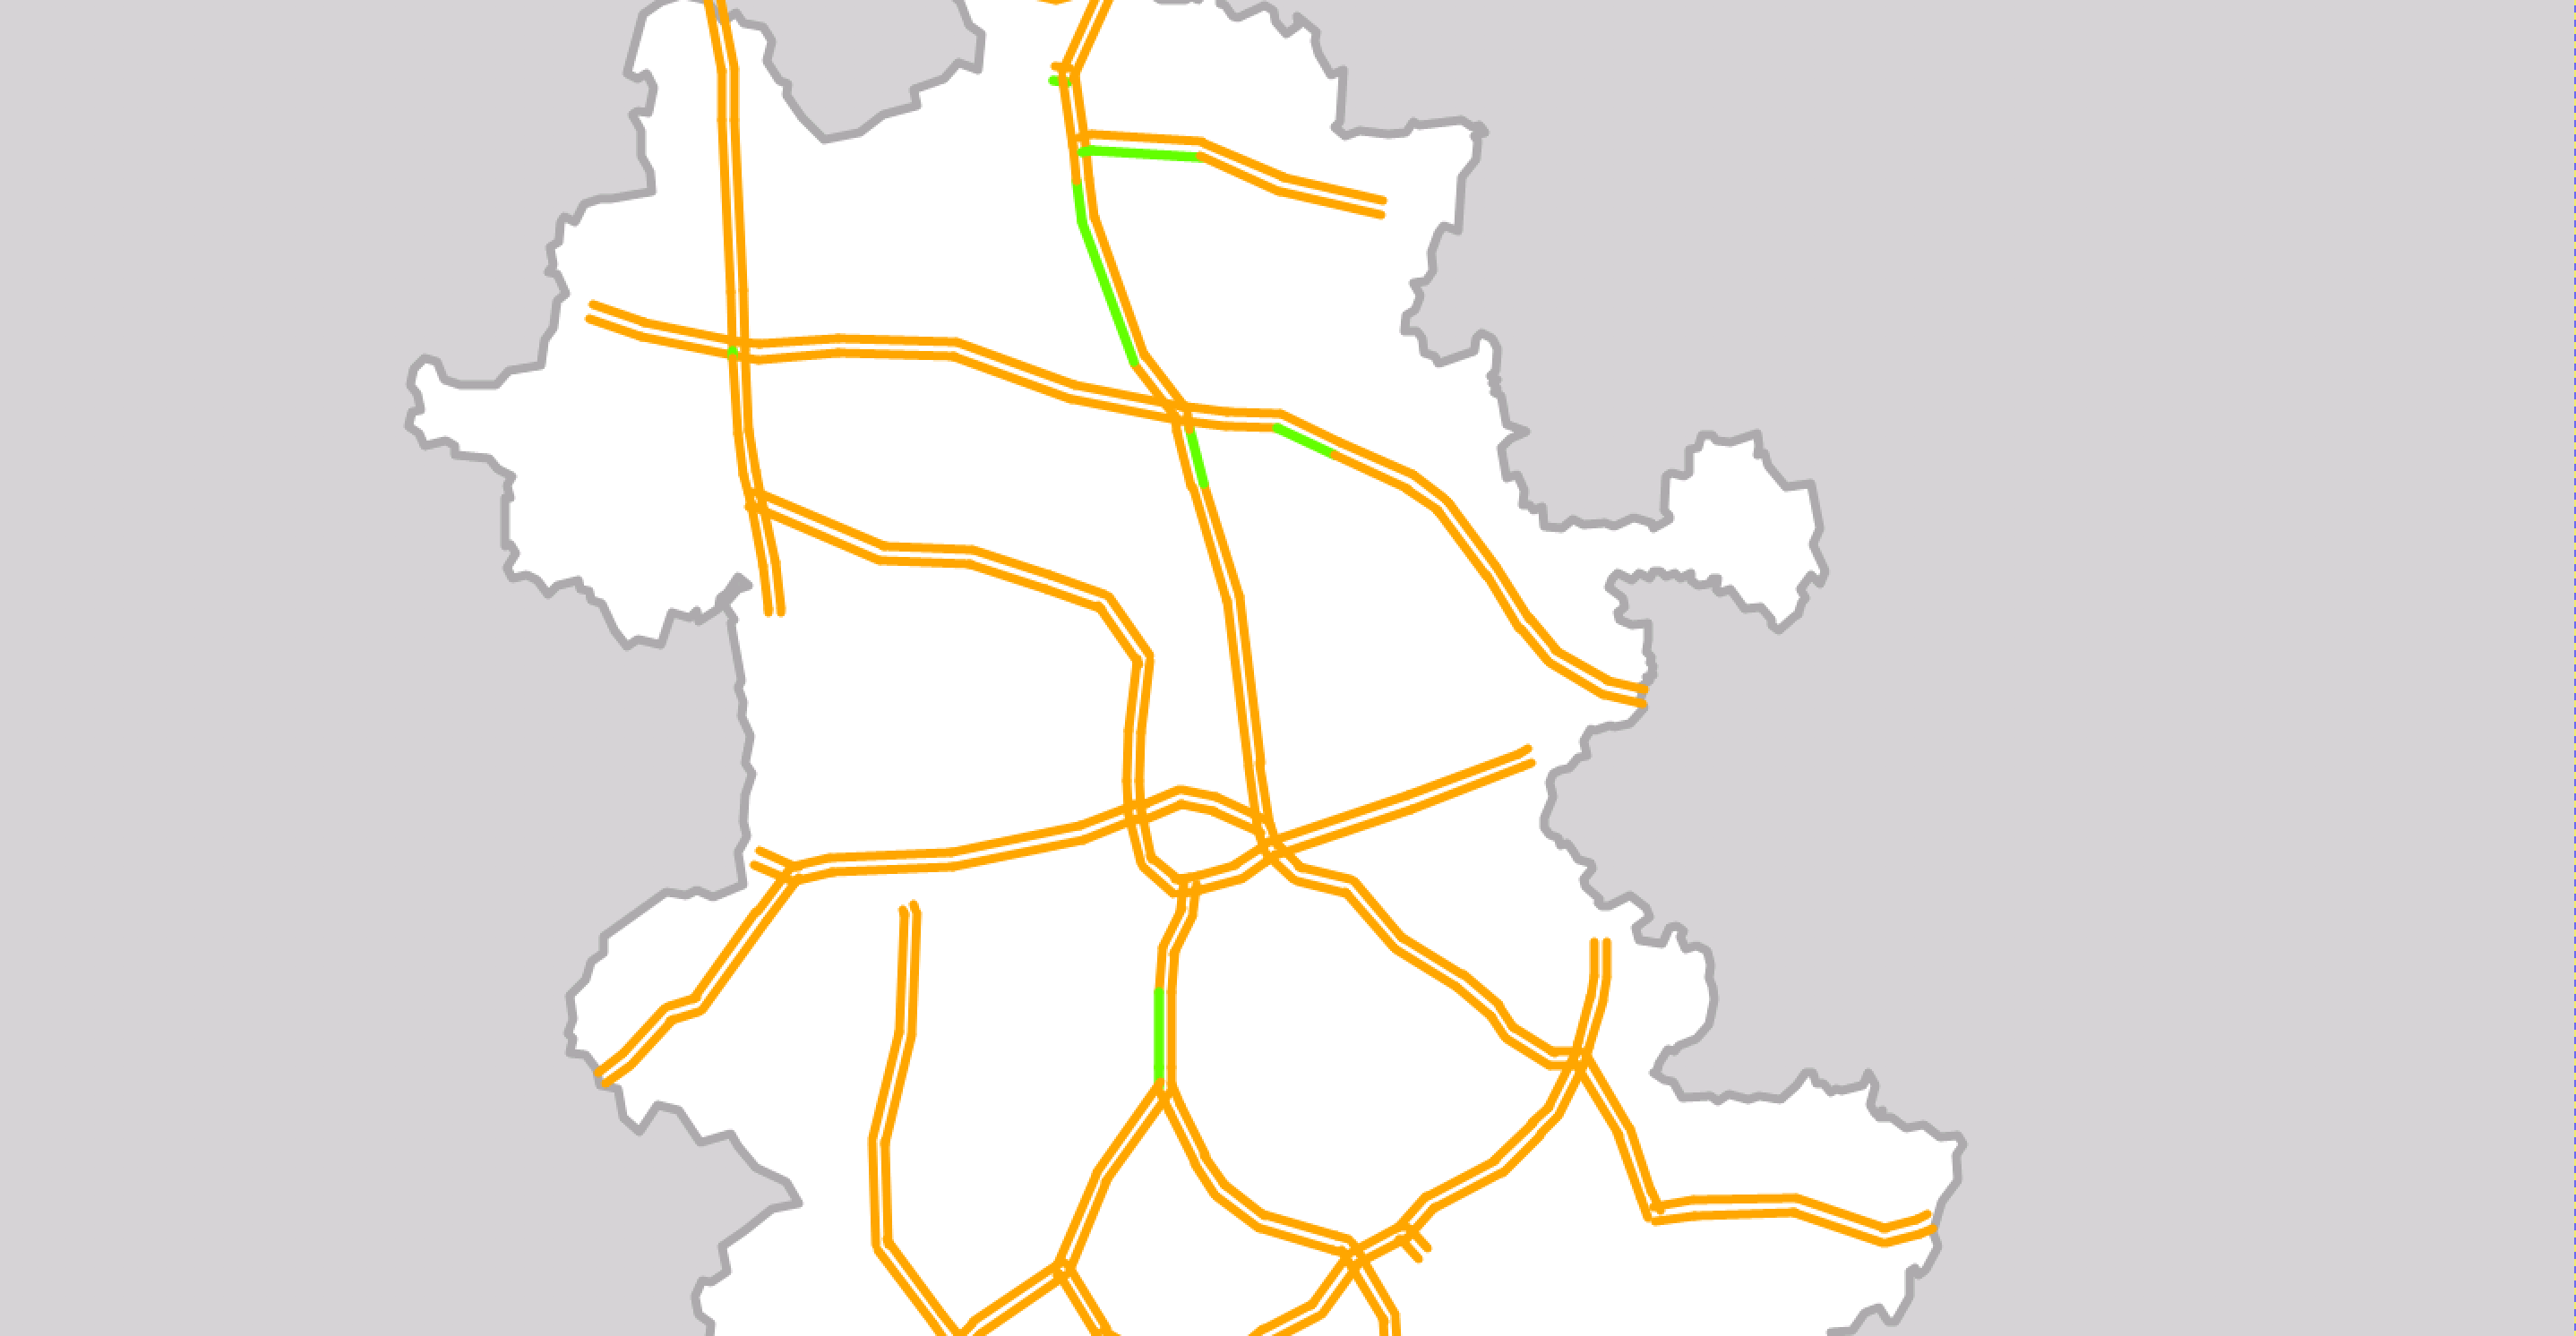
\includegraphics[width=3in]{picture/fenqun}
					\caption{基于社群划分的关键路段}
					\label{jihe3}
				\end{minipage}%
				\begin{minipage}{0.5\linewidth}
					\centering
					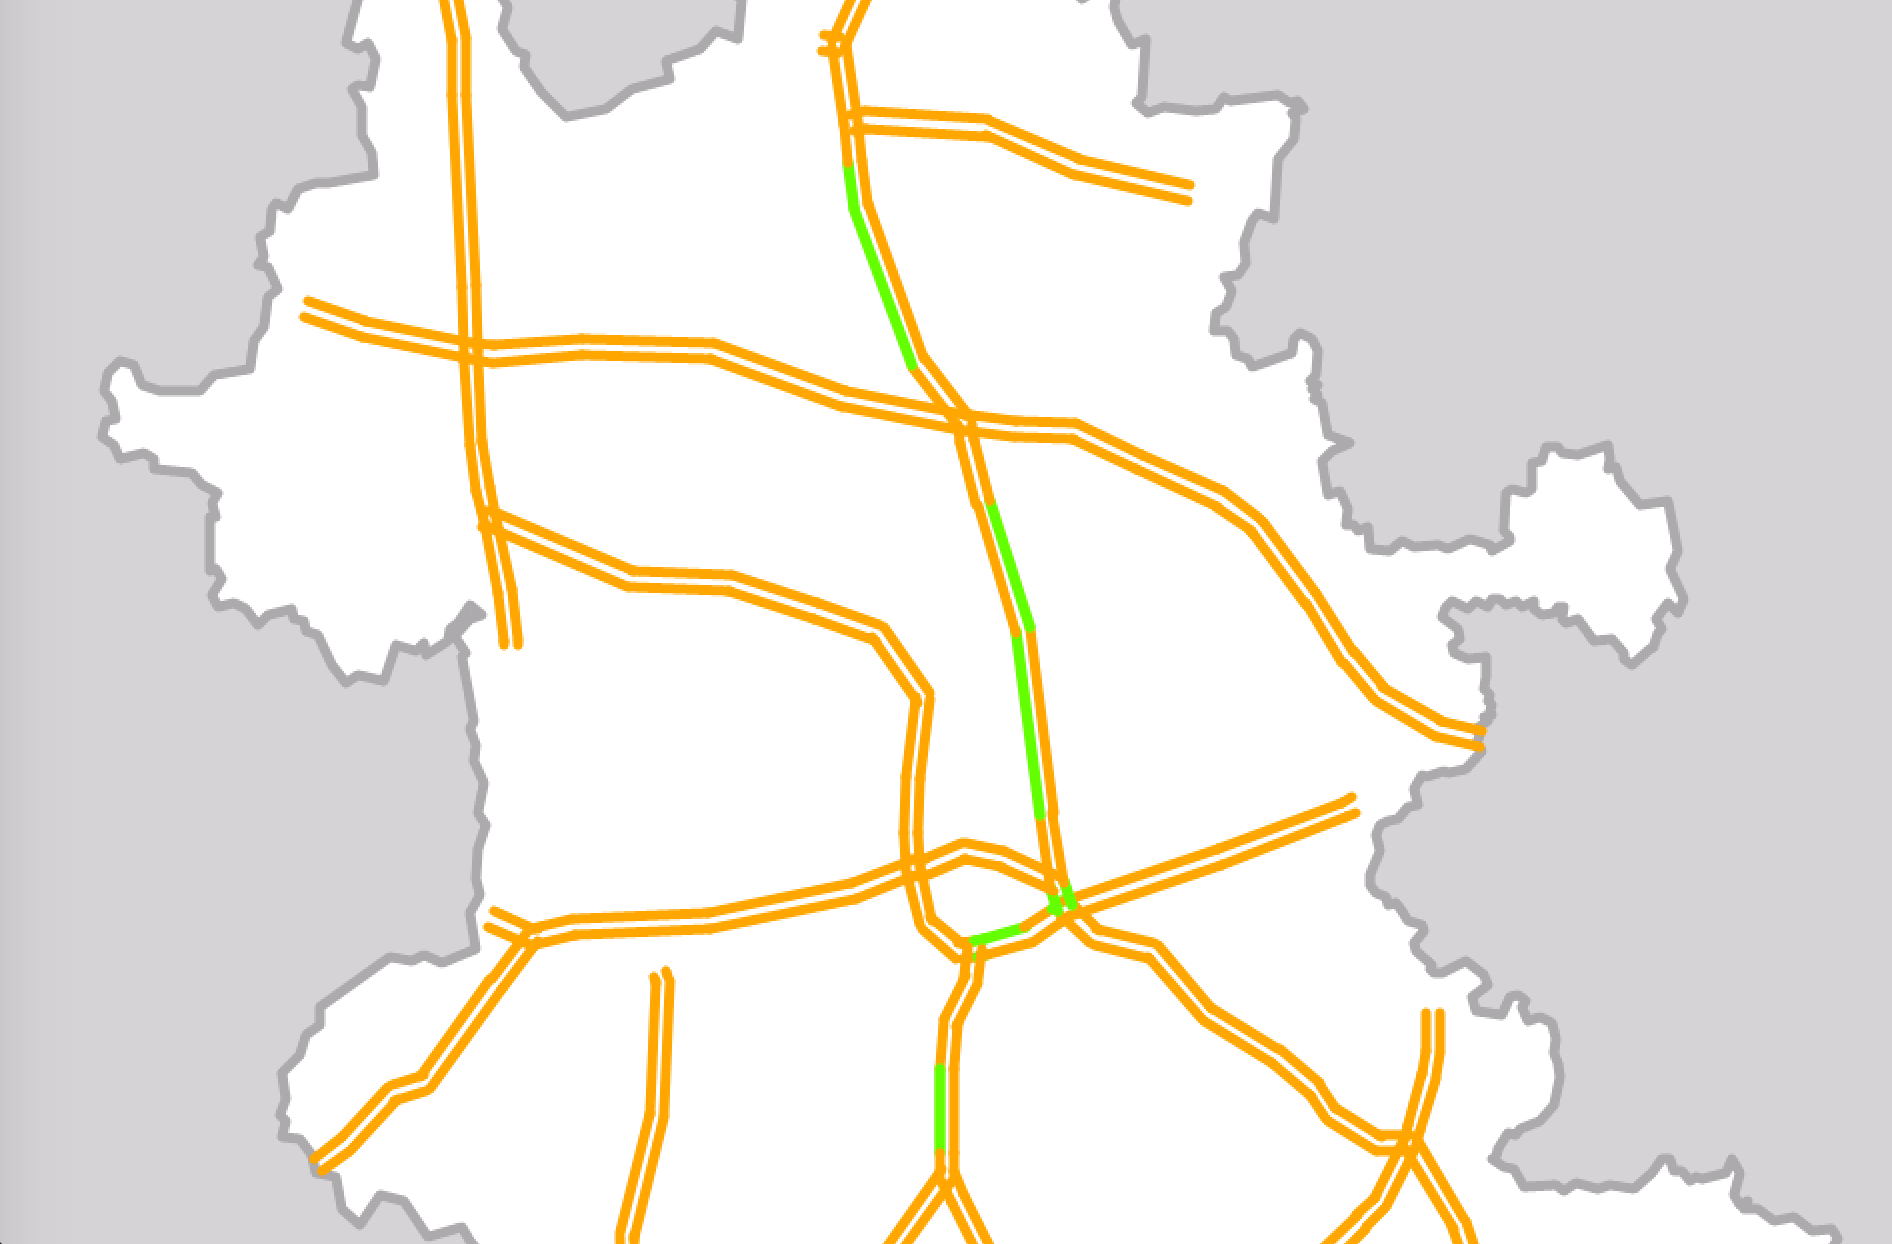
\includegraphics[width=2.5in]{picture/hotsection}
					\caption{基于统计学的关键路段}
					\label{jihe4}
				\end{minipage}
				\end{figure}

		误差分析:

				\begin{table}[h]
				\centering
				\begin{tabular}{|c|c|c|}
				\hline
				\hline
				  &  枚举-直接贪心 &  直接贪心-基于社群划分 \\
				\hline
				 一小时 &  14.63\% &  12.89\% \\
				\hline
				 一天 &  13.25\% &  13.26\% \\
				\hline
				 一周 &  13.10\% &  15.61\% \\
				\hline
				 一月 &  12.99\% &  11.59\% \\
				\hline
				\end{tabular}
				\caption{路网通行效率提升量误差分析}
				\label{table1}
				\end{table} 

		表\ref{table1}描述了枚举方法和直接贪心方法之间的误差,直接贪心和基于社群划分方法之间的误差。误差由高速路网的通行效率计算,可以看出误差在允许范围内。

		关键路段选取平均误差:

				\begin{table}[h]
				\centering
				\begin{tabular}{|c|c|c|}
				\hline
				\hline
				   &   枚举-直接贪心 &   枚举-基于社群划分 \\
				\hline
				  一小时 &   0.18 &   0.25\% \\
				\hline
				  一天 &   0.14\% &   0.20\% \\
				\hline
				  一周 &   0.15\% &   0.19\% \\
				\hline
				  一月 &   0.14\% &   0.17\% \\
				\hline
				\end{tabular}
				\caption{关键路段选取误差分析}
				\label{table2}
				\end{table} 

		表\ref{table2}分析了关键路段选取情况的误差,采用欧式距离来刻画区别。可以看出,随着数据集的扩大,基于社群划分方法的关键路段准确率逐步上升。

		运行效率分析:

				\begin{table}[h]
				\centering
				\begin{tabular}{|c|c|c|c|c|}
				\hline
				\hline
				   &   枚举 &   直接贪心 &   基于社群划分 &   基于统计 \\
				\hline
				  一小时 &   1day &   30min &   2min &   1min \\
				\hline
				  一天 &   6day &   2h &   5min &   2min \\
				\hline
				  一周 &  7day &   3h &   6min &   5min \\
				\hline
				  一月 &   7day &   3h &   7min &   8min \\
				\hline
				\end{tabular}
				\caption{不同方法运行效率分析}
				\label{table3}
				\end{table} 

		由表\ref{table3}可以看出,基于社群划分方法可以将整个算法的时间复杂度再降一个数量级,而结合表\ref{table1}来看,精度误差处于可接受范围$(1/e)$。

	\section{本章小结}
		本章提出了面向高速公路的社群划分方法,首先分析了传统方法的局限性,然后结合高速公路的独有特性,采用多变权值-模拟退火结合的方法,实现符合高速公路网络特点的社群划分方法。最后结合动态规划方法,实现多项式时间求解。